% 
% Template file for software architecture design description in the 
% DIKU course Software Architecture and Software Design. Please do
% not distribute outside the course
% 
% Based on a template (c) by Woods and Rozanski (2011) available at
% 
%    http://www.viewpoints-and-perspectives.info
% 
% Instructions:
%
% 1) change the metadata commands below (\groupname) etc. to fit your
%     project
% 2) uncomment the overwriting of the \instructions command to remove 
%     instructions
% 3) write your architectural description...
%
% Contact: klausmh@diku.dk
% 
\documentclass[a4paper,11pt]{report}
\usepackage{natbib}
\usepackage[pdftex]{graphicx}
\usepackage{color}
\usepackage[table]{xcolor}
\usepackage{hyperref}
\usepackage{lastpage} 

% Meta-data for report
\newcommand{\systemname}{Siberian Trucking System}
\newcommand{\groupname}{Lima}
\newcommand{\contactdetails}{athas@sigkill.dk, shantanubala@gmail.com, jesper\_tved@hotmail.com}

% Typesetting of instructions for using the template,
% remove by renewing command 
\newcommand{\instructions}[1]{
  \noindent\colorbox{lightgray}{%
    \parbox{\linewidth}{%
      #1
    }%
  }%
 \vspace{0.1cm}
}
% \renewcommand{\instructions}[1]{} % Uncomment to remove instructions

% We use the below command for figure captions since
% the figure environment does not play nicely with 
% \colorbox. The "real" way to create figures is like this:
%   \begin{figure}[ht!]
%     \centering
%     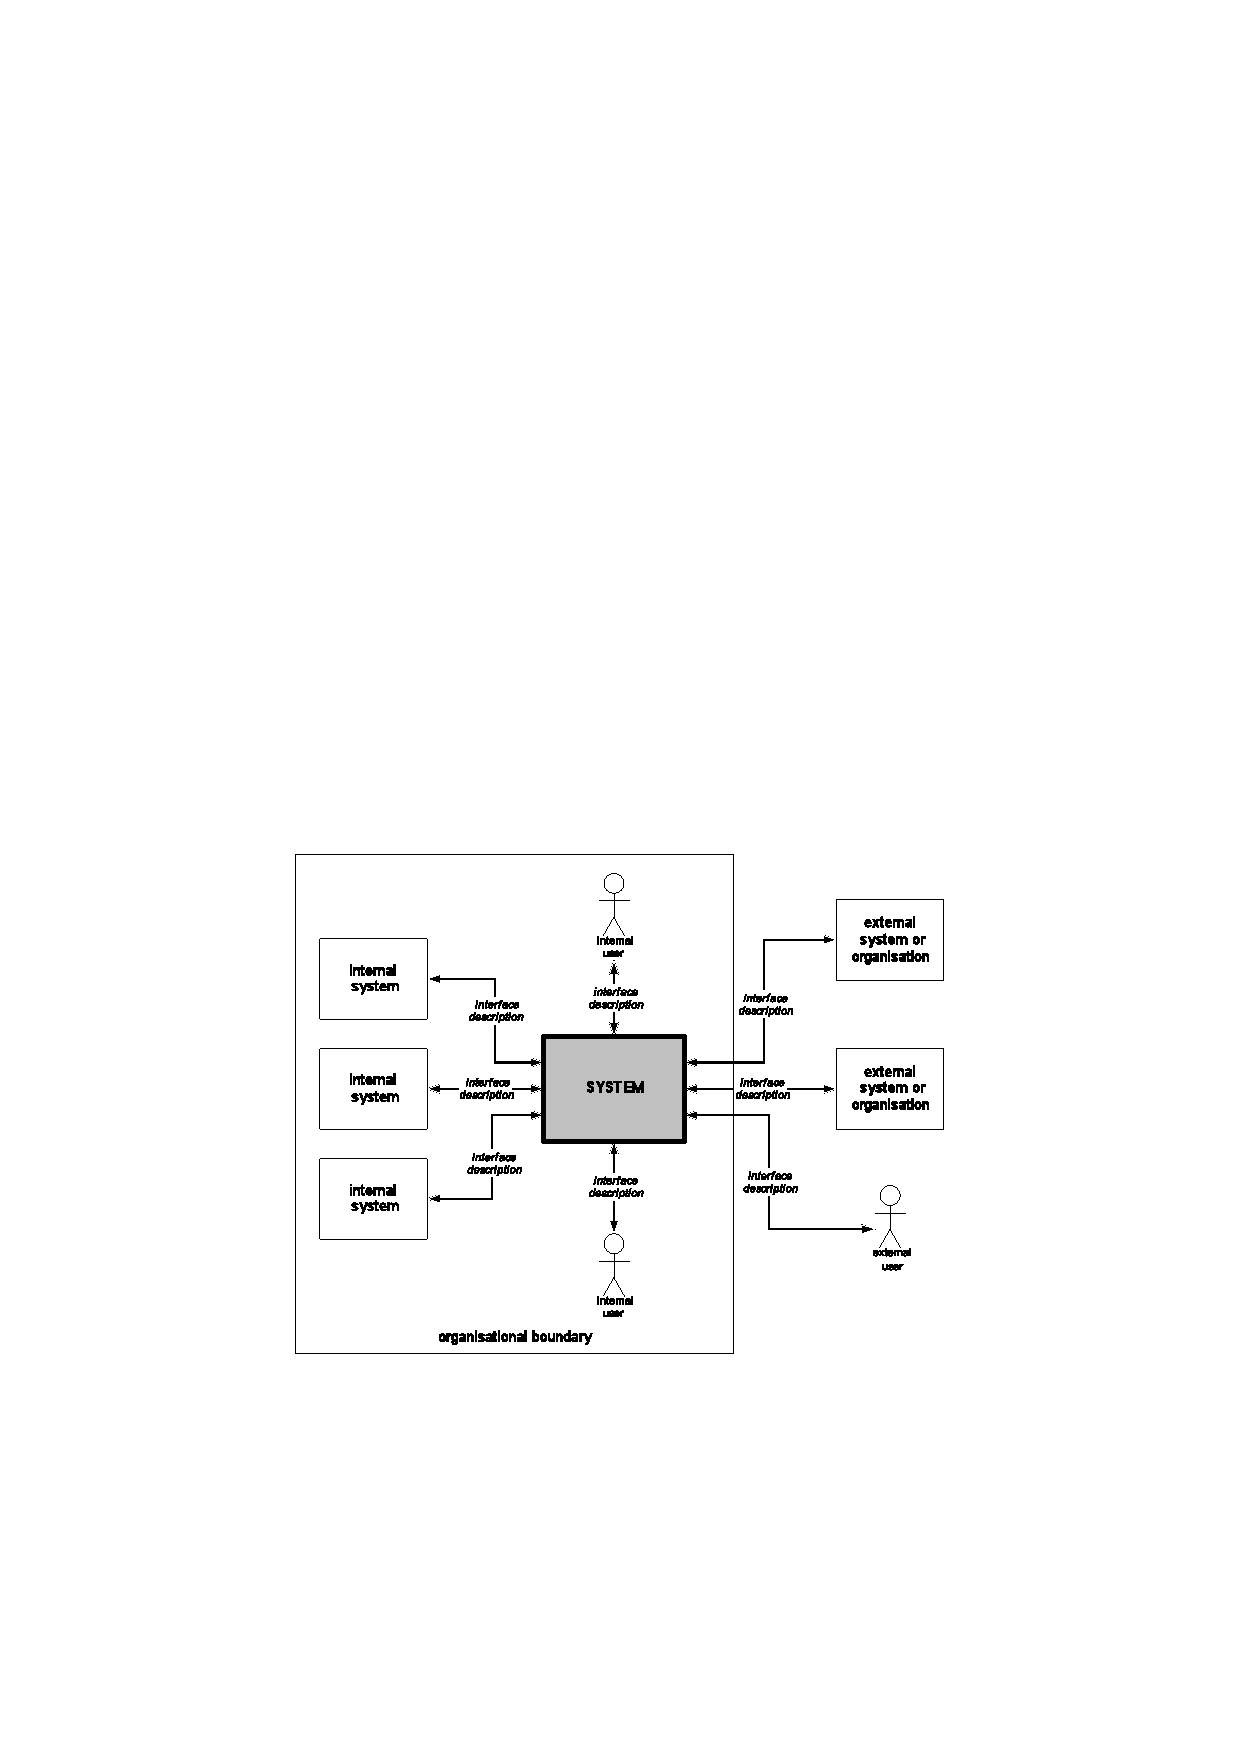
\includegraphics[width=0.8\textwidth]{figures/systemcontext}
%    \caption{System context}
%     \label{fig:systemcontext}
%   \end{figure}
\newcommand{\mycaption}[1]{
  \addtocounter{figures}{1}
  Figure \arabic{figures}. #1
}

% Change font family to Helvetica
\renewcommand{\rmdefault}{phv}
\renewcommand{\sfdefault}{phv}

% Set headers and footers
\usepackage{fancyhdr}
\pagestyle{fancy}
\fancyhf{}
\fancyhead[C]{Software Architecture of \systemname\ }
\fancyfoot[C]{\footnotesize Page \thepage\ of \pageref{LastPage}}


\begin{document}
% 
% Title page
% 
\newcommand{\HRule}{\rule{\linewidth}{0.5mm}}
\begin{titlepage}

  \begin{center}

    % Title
    \vspace*{4cm}
    \HRule \\[0.4cm]
    { \huge \bfseries \systemname}\\[0.4cm]
    \HRule \\[1.5cm]

    {\Large Software Architecture Description}

    \vfill
  \end{center}

  % Author, version, date
  \begin{flushleft}
    {\large \groupname}\\[0.2cm]
    {\large \contactdetails}\\[0.2cm]
   {\large \today}
  \end{flushleft}
\end{titlepage}

% 
% Version table
% 
\newpage
\chapter*{Version history}

\begin{center}
  \begin{tabular}[h!]{| l | l | l | p{8 cm} |}
    \hline
    \rowcolor{gray}
    Version & Date & Author & Comments \\
    \hline
    \hline
    1 & 2012-08-17 & KMH & Initial template based on
    \citep{rozanski2011software} \\
    \hline
    2 & 2012-09-10 & JTM & added 1.1, 1.2, 1.3 and 5.1 \\
    \hline
    & & & \\
    \hline
  \end{tabular}
\end{center}

% 
% Table of contents
% 
\setcounter{tocdepth}{1}
\tableofcontents

% 
% Main text
% 
\chapter{Introduction}
\label{cha:introduction}
\thispagestyle{fancy}

\instructions{Text typeset like this in an instruction on how to use
  the template. They should (of course) be removed in an architectural
  description. 

  In the LaTeX file for the template, this can be done by renewing the
  \texttt{{\textbackslash}instructions} command to output the empty string.
}

\section{Purpose and scope}
\label{sec:purpose-scope}

Russia, as the worlds largest country by land area, has an extensive
raw materials industry.  Since the fall of the Soviet Union, the
Russian trucking industry has undergone a dramatic growth, and
government initiatives aim to maintain this growth into the future.
Since many of the industrial installations are located in remote
areas, logistics companies face great difficulties in managing their
truck fleets, particularly as transportation times are often
unpredictable due to weather, accidents and the generally poor
condition of the Russian road network.  As an additional complication,
the distant locations and low population densities prevents the use of
many common communication technologies (eg. no cell phone network).

We propose the creation of a system, the Siberian Tracking System
(STS), for tracking a large fleet of trucks operating in far-flung
regions of Russia, owned by the (fictive) Siberian Trucking Company
(STC).  A central server installation will be informed of the location
and state of every truck in the fleet, permitting decision making
systems to have complete knowledge of the state of the company assets.
Each truck is responsible for tracking its own progress, then
periodically relaying it back to the main servers.  The project does
not involve creation of any new ground stations; trucks will use
standard wireless communication methods whenever in range of
appropriate networks. The transmitters on the trucks will only use one way communication to the server, with data of the trucks current position and the speed of the truck. The transmitters are supposed to be low-cost hardware, so communication from the server to the trucks and additional measuring equipment, for instance of oil and gasoline levels have been deselected. 

The STS is solely concerned with the state of the trucking fleet, and
does not do freight tracking or make any kind of business logic
decisions on its own.  While it provides information allowing such
decisions to be made, it is purely a data collection and dissemination
infrastructure.  In particular, it is a one-way communication system.
Other means must be employed to contact the trucks on the road.  Also,
STS is by itself not concerned with doing data mining or presenting a
sophisticated user interface to its data.  Instead, a data interchange
mechanism will be defined that allows other systems to receive
information from STS.

\section{Audience}
\label{sec:audience}

The intended audience of this document, and the reason for their
inclusion, are as follows.

\begin{itemize}
  \item Business logic decision makers of STC, who must determine
    whether the information provided by STS is sufficient.
  \item Truck maintenance department representatives, to determine
    whether the additional equipment needed on trucks is realistic.
  \item The developers who have to implement the suggested architecture and design.
  \item Finally, whoever approves the financing of the project.
\end{itemize}

\section{Status}
\label{sec:status}

The basic requirements of STS have been determined, but the actual
design and implementation is not yet begun.

\section{Architectural design approach}
\label{sec:arch-design-appr}

\instructions{
  Explain the overall architectural approach used to describe and
  develop the content of the document (e.g. explain viewpoints, views
  and perspectives). If necessary explain the architectural views that
  you’re using and why each is used.
}

\chapter{Glossary}
\label{cha:glossary}
\thispagestyle{fancy}

\begin{center}
  \begin{tabular}[h!]{| p{0.2\textwidth} | p{0.7\textwidth} |}
    \hline
    \rowcolor{gray}
    Term & Definition \\
    \hline
    \hline
    Mesh network & An ad-hoc (usually short-range) network formed by autonomous units within range of each other \\\hline
    STS & Siberian Tracking System.  Refers both to the project as a whole, and to the software running on stationary servers (ie. excluding the software on truck transmitters). \\\hline
    STC & Siberian Tracking Company \\\hline
    Truck transmitter & The hardware unit on a truck.  Consists of a GPS receiver and an antenna for communications. \\\hline
  \end{tabular}
\end{center}

\chapter{System stakeholders and requirements}
\label{cha:syst-stak-requ}
\thispagestyle{fancy}

\section{Stakeholders}
\label{sec:stakeholders}

\begin{itemize}
  \item Acquirers: the Siberian Trucking Company (STC) will be paying for the
    development of the system to aid in business logic. The users of the system
    will be members of the STC's business administration.
  \item Communicators: the technical writers who will create documentation regarding the
    operation of the system, while the business administration of the STC will
    be responsible for the training of the end users of the system.
  \item Developers: the STC has contracted a group from the University of
    Copenhagen to develop the system.
  \item Maintainers: the STC has a team of developers responsible for
    maintaining and evolving the STS system after it is completed.
  \item Production Engineers: the STS system will be deployed onto the Amazon
    EC2 platform, outsourcing the deployment environment to Amazon's
    engineering staff.
  \item Suppliers: servers will be provided by Amazon's EC2 platform, while the
    GPS units are assumed to already be installed on the STC's trucks.
  \item Support Staff: it is assumed that the STC has the appropriate IT staff
    for helping the end users of the STS in accomplishing their appropriate
    business administration tasks.
  \item System Administrators: Amazon provides the appropriate hardware
    administration while the STC has a team of developers responsible for
    updating and maintaining the software environment of the EC2 instances.
  \item Testers: The STC has a team of developers responsible for testing and
    ensuring the STS works effectively.
  \item Users: members of the STC's business administration team who will use
    and analyze data provided by the STS to make informed business decisions.
\end{itemize}

\section{Overview of requirements}
\label{sec:overv-requ}

\begin{center}
  \begin{tabular}[h!]{| p{0.2\textwidth} | p{0.7\textwidth} |}
    \hline
    \rowcolor{gray}
    Reference & Requirement description \\
    \hline
    \hline
    R1 & The system must provide business administrators with a detailed
    history of the location of every truck in the STC fleet. \\
    \hline
    R2 & The system must be able to receive and store 1,000 GPS datapoints per
    second. \\
    \hline
    R3 & The server interface for storing the trucks' location data must have
    an availability of at least 99 percent uptime. \\
    \hline
    R4 & The tracking units present on each of the trucks must have a fallback
    when data cannot be sent in real-time due to bad network coverage. \\
    \hline
    R5 & The server interface must be capable of receiving an individual data
    point (the truck's location) or a series of data points (the truck's
    location history over a period of time). \\
    \hline
  \end{tabular}
\end{center}

\section{System scenarios}
\label{sec:system-scenarios}

\subsection{Functional scenarios}
\label{sec:functional-scenarios}

\begin{center}
  \begin{tabular}[h!]{| >{\columncolor{gray}}p{0.28\textwidth} | p{0.65\textwidth} |}
    \hline
    Scenario reference & FS1. \\
    \hline
    Overview & How truck information is sent to the server \\
    \hline
    System state & The truck is fitted with a truck transmitter and is currently driving\\
    \hline
    System environment & The system is operating normally\\
    \hline
    External stimulus & The truck transmitter has a position that should be sent to the server\\
    \hline
    Required system response & If the truck is in range of a network, the position is sent to the server and a confirmation is received. If the truck is out of range, the position is stored in the truck transmitter and will be sent when the truck is in range of a network again \\
    \hline
  \end{tabular}
\end{center}

\begin{center}
  \begin{tabular}[h!]{| >{\columncolor{gray}}p{0.28\textwidth} | p{0.65\textwidth} |}
    \hline
    Scenario reference & FS2. \\
    \hline
    Overview & How truck positions are queried by a user \\
    \hline
    System state & Positions from many different trucks have been sent to the server with timestamps\\
    \hline
    System environment & The system is operating normally\\
    \hline
    External stimulus & The user queries a specific truck, trucks within an area, and trucks that have not yet reached their deignated targets on time\\
    \hline
    Required system response & The system shows the requested data as a list in the users GUI \\
    \hline
  \end{tabular}
\end{center}

\begin{center}
  \begin{tabular}[h!]{| >{\columncolor{gray}}p{0.28\textwidth} | p{0.65\textwidth} |}
    \hline
    Scenario reference & FS3. \\
    \hline
    Overview & New trucks are imported to the system \\
    \hline
    System state & New trucks are listed in the truck registry and a transmitter have been fitted into the new truck\\
    \hline
    System environment & STS, the truck transmitter and the truck registry is operating normally\\
    \hline
    External stimulus & An employee from the support staff have registered the truckID with the trucks transmitterID \\
    \hline
    Required system response & STS can now be queried for the new trucks ID \\
    \hline
  \end{tabular}
\end{center}

\begin{center}
  \begin{tabular}[h!]{| >{\columncolor{gray}}p{0.28\textwidth} | p{0.65\textwidth} |}
    \hline
    Scenario reference & FS4. \\
    \hline
    Overview & How transmittion network are chosen \\
    \hline
    System state & The truck is fitted with a truck transmitter and is currently driving\\
    \hline
    System environment & The truck transmitter and the truck registry is operating normally, the truck is driving in an area without any connection\\
    \hline
    External stimulus & The truck transmitter has a new position that should be sent to the server \\
    \hline
    Required system response & The truck transmitter first tries to send via GSM mobile network, after this the long range mesh-network is tried. If neither of these worked, the position is stored to be sent at a later point. \\
    \hline
  \end{tabular}
\end{center}

\subsection{System quality scenarios}
\label{sec:syst-qual-scen}

\begin{center}
  \begin{tabular}[h!]{| >{\columncolor{gray}}p{0.28\textwidth} | p{0.65\textwidth} |}
    \hline
    Scenario reference & QS1. \\
    \hline
    Overview & If the number of trucks in the fleet increases, or if the business
    administrators need to collect data at a greater interval, the capabilities
    of the system ought to be appropriately scalable.\\
    \hline
    System environment & This process will be handled
    by Amazon's Elastic Load Balancing service in conjunction with Amazon EC2.\\
    \hline
    Environment changes & For example, if 10 small EC2
    instances can receive and process 1,000 data points per second, the system will
    allocate the equivalent of 50 small EC2 instances to process an increased
    workload of 5,000 data points per second.\\
    \hline
    Required system behavior & When a tracking device in
    a truck sends data to the STS server, the data will be placed in a queue.
    Based on the size of the queue, an appropriate number of EC2 instances will
    be started or shut down to process the queue.\\
    \hline
  \end{tabular}
\end{center}

\begin{center}
  \begin{tabular}[h!]{| >{\columncolor{gray}}p{0.28\textwidth} | p{0.65\textwidth} |}
    \hline
    Scenario reference & QS2. \\
    \hline
    Overview & If the cellular network is not available, the transmitter on the
    truck will fall back to using a long-distance mesh network established
    between the trucks. \\
    \hline
    System environment & This process will be handled
    by the transmitters that are installed on every truck in the STC fleet.\\
    \hline
    Environment changes & For example, if a truck leaves cell network range, it
    will attempt to connect to a nearby truck, which will also be connected to
    other trucks. As long as a single truck in the mesh has cell coverage, all
    of the trucks will be able to transmit their data.\\
    \hline
    Required system behavior & The trucks' transmitters will have a queue for
    sending data to the STS server, and will process this queue using the
    fastest available connection.\\
    \hline
  \end{tabular}
\end{center}

\begin{center}
  \begin{tabular}[h!]{| >{\columncolor{gray}}p{0.28\textwidth} | p{0.65\textwidth} |}
    \hline
    Scenario reference & QS3. \\
    \hline
    Overview & If part of the Amazon EC2 cluster fails, the error must not propagate to the entire system.\\
    \hline
    System environment & This robustness must be built into the software running on the EC2 cluster.  Additionally, the truck transmitters must still be able to transmit data. \\
    \hline
    Environment changes & If a node in the cluster loses contact with another node, it must ensure that the overall system still has redundant data, such that further node failures can be handled.  The trucks must be able to connect to another node if the usual recipient for their data fails to respond.  If the system is sufficiently heavily damaged that data integrity is lost, it must still be possible for trucks to transmit data, but any queries in the data should have their result marked as incomplete.  \\
    \hline
    Required system behavior & Heavy data redundancy must be built into the system.  Whenever a truck reports back, it may also receive an updated list of communication endpoints. \\
    \hline
  \end{tabular}
\end{center}

\begin{center}
  \begin{tabular}[h!]{| >{\columncolor{gray}}p{0.28\textwidth} | p{0.65\textwidth} |}
    \hline
    Scenario reference & QS4. \\
    \hline
    Overview & If the transmitter on a truck fails, this failure must be noticed and rectified. \\
    \hline
    System environment & The system must have logic to detect when a truck ``should'' have transmitted information, but has not.  We assume that the fabrication and installation of new transmitters is done externally of our system. \\
    \hline
    Environment changes & If a truck fails to report back, the maintenance department must be notified that a truck has a faulty transmitter, and that it must be replaced. \\
    \hline
    Required system behavior & We receive information from the truck register whenever the truck reaches some central locations.  If the truck itself does not send the same information, its transmitter will be assumed defective, and called in for repair.  As long as every truck is guaranteed to eventually stop at such a destination, any failure will eventually be discovered. \\
    \hline
  \end{tabular}
\end{center}

\chapter{Architectural forces}
\label{cha:architectural-forces}
\thispagestyle{fancy}

\section{Goals}
\label{sec:goals}

\begin{description}
\item[Business driver:] Trucking in Russia is mostly done using old and inefficient
  trucks with bad road conditions.  It is not feasible to replace the
  vehicles or the road system, so in order to remain competetive, the
  STC must optimise its logistics intead.
\item[Project goal:] The STC wishes to optimise its logistics by
  keeping a detailed log of truck movement.  By analysing the
  information the log, more efficient transportation routes may be
  designed.
\item[Project goal:] In order to minimise truck idle time, the STC
  desires real-time information on truck locations, such that
  availability for further use can be easily predicted.
\end{description}

\section{Constraints}
\label{sec:constraints}

\begin{itemize}
\item The company has very little in-house IT capacity, and does not
  wish to expand it much.  In particular, it does not want to maintain
  its own servers.
\item Since the servers must consequently be outsourced, the STS has
  to run in a generic, non-customised environment (such as a standard
  Linux server).
\item The truck transmitters are very restricted, embedded hardware,
  that cannot run large and complicated software.
\item Trucking in Russia is at an unusually high risk of hijacking.
  In order to not leak information about the locations of trucks, all
  communications has to be protected from eavesdropping, and all
  queries in the database must be authorised.
\item As another safety-related concern, it must not be possible for a
  third party to falsify truck information.
\end{itemize}

\section{Architectural principles}
\label{sec:arch-princ}

\begin{center}
  \begin{tabular}[h!]{| >{\columncolor{gray}}p{0.28\textwidth} | p{0.65\textwidth} |}
    \hline
    Principle reference & P1. \\
    \hline
    Principle statement & Redundancy of components \\
    \hline
    Rationale & The STS will be of critical importance in making real-time business decisions, so it is important that it is always available. \\
    \hline
    Implications & \begin{itemize}
      \item System distributed across multiple nodes (for example, using multiple different Amazon EC2 instances across multiple availability zones).
      \item Comprehensive error handling in all levels of the system.
      \item Load balancing to handle node failures.
      \item Redundancy at the data level, for example through replication.
      \end{itemize}
        \\
    \hline
  \end{tabular}
\end{center}
\begin{center}
  \begin{tabular}[h!]{| >{\columncolor{gray}}p{0.28\textwidth} | p{0.65\textwidth} |}
    \hline
    Principle reference & P2. \\
    \hline
    Principle statement & Use of open source components \\
    \hline
    Rationale & Open source components will be used where available, in order to reduce development effort and cost. \\
    \hline
    Implications & \begin{itemize}
      \item Able to modify external components, if necessary.
      \end{itemize}
        \\
    \hline
  \end{tabular}
\end{center}
\begin{center}
\begin{tabular}[h!]{| >{\columncolor{gray}}p{0.28\textwidth} | p{0.65\textwidth} |}
    \hline
    Principle reference & P3. \\
    \hline
    Principle statement & Encryption of communications \\
    \hline
    Rationale & To prevent outsiders from gaining knowledge about truck locations, all communications across external networks must be encrypted \\
    \hline
    Implications & \begin{itemize}
      \item An encryption scheme must be decided upon.
      \item We don't have to worry about security of the link layers.
      \end{itemize}
        \\
    \hline
  \end{tabular}
\end{center}
\begin{center}
\begin{tabular}[h!]{| >{\columncolor{gray}}p{0.28\textwidth} | p{0.65\textwidth} |}
    \hline
    Principle reference & P4. \\
    \hline
    Principle statement & Cryptographic signing of truck communications \\
    \hline
    Rationale & To prevent third parties from impersonating truck transmitters, all communications from trucks must be signed using assymetric cryptography. \\
    \hline
    Implications & \begin{itemize}
    \item The cryptographic keys must be managed.
    \item If a key is leaked, there must be a procedure for changing them.
    \end{itemize}
        \\
    \hline
  \end{tabular}
\end{center}
\begin{center}
\begin{tabular}[h!]{| >{\columncolor{gray}}p{0.28\textwidth} | p{0.65\textwidth} |}
    \hline
    Principle reference & P5. \\
    \hline
    Principle statement & The information retrieval API is REST-oriented \\
    \hline
    Rationale & REST APIs are easy to interface with existing HTTP protocol stacks. \\
    \hline
    Implications & \begin{itemize}
    \item We need visible HTTP servers.
    \item A protocol for how to represent the data in textual form
      must be decided.
    \end{itemize}
        \\
    \hline
  \end{tabular}
\end{center}
\begin{center}
\begin{tabular}[h!]{| >{\columncolor{gray}}p{0.28\textwidth} | p{0.65\textwidth} |}
    \hline
    Principle reference & P6. \\
    \hline
    Principle statement & Communication from trucks to STS is one-way only \\
    \hline
    Rationale & The trucks may often not communicate directly, but relay their information via a mesh network \\
    \hline
    Implications & \begin{itemize}
    \item Trucks cannot adapt their behavior in response to actions taken by the system.
    \item We can use batched, asynchronous communications.
    \end{itemize}
        \\
    \hline
  \end{tabular}
\end{center}
\begin{center}
\begin{tabular}[h!]{| >{\columncolor{gray}}p{0.28\textwidth} | p{0.65\textwidth} |}
  \hline
  Principle reference & P7. \\
  \hline
  Principle statement & Mesh networking by trucks \\
  \hline
  Rationale & In order to extend range beyond cell phone networks, short-range mesh networks between truck transmitters is used to indirectly transmit to STS. \\
  \hline
  Implications & \begin{itemize}
  \item A truck can relay information about any number of other trucks.
  \item Every piece of truck communication must be identified by the
    original sender, not the truck that managed to contact the STS.
    \end{itemize}
        \\
    \hline
  \end{tabular}

\end{center}

\chapter{Architectural views}
\label{cha:architectural-views}
\thispagestyle{fancy}

\section{Context view}
\label{sec:context-view}

\newcounter{figures}

\begin{center}
  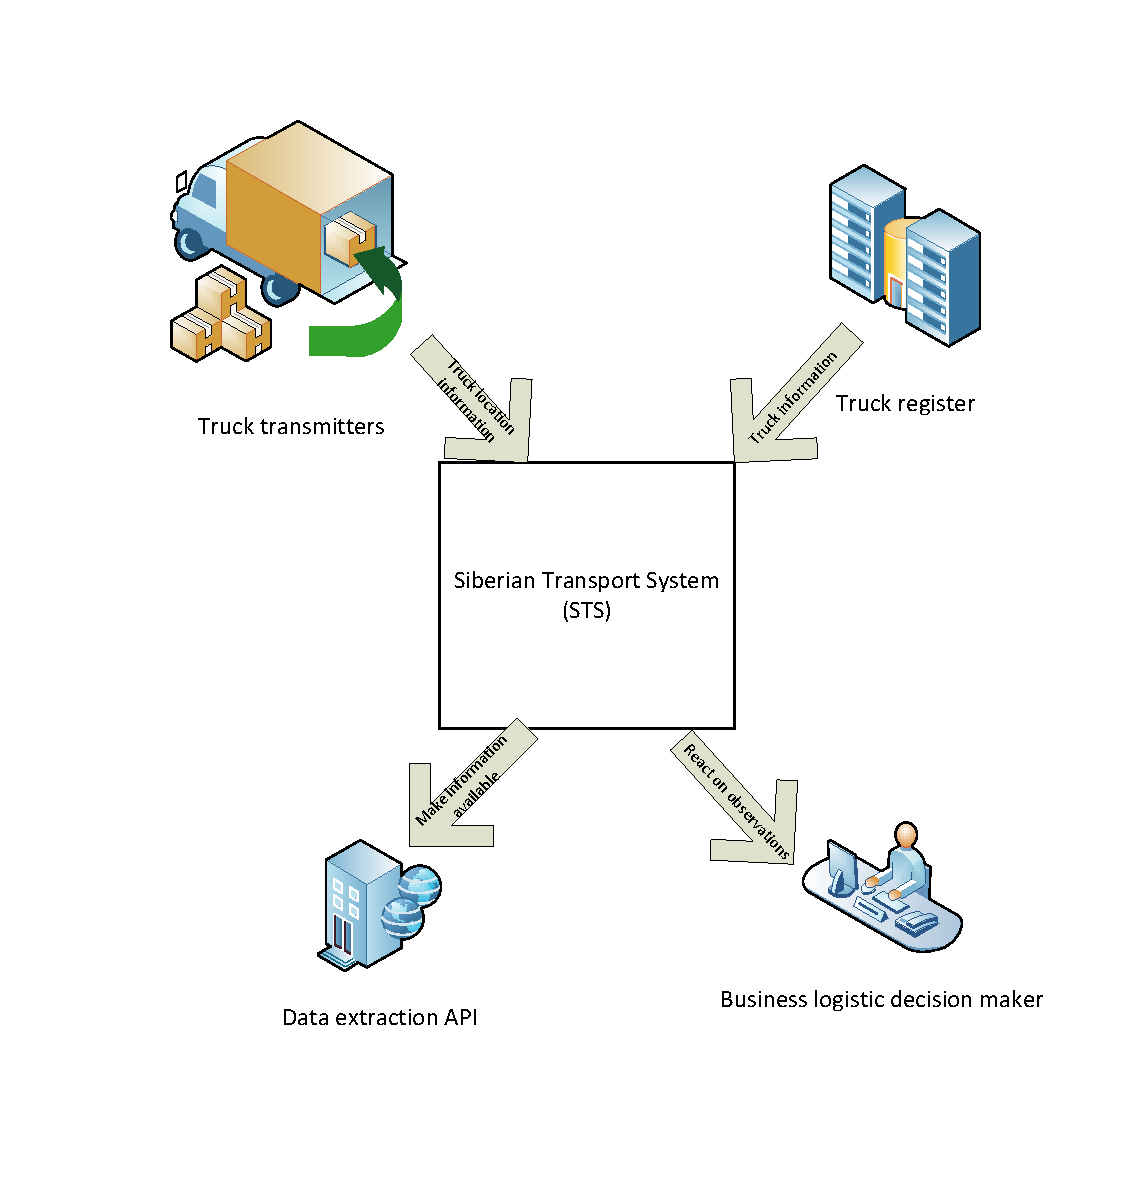
\includegraphics[width=\textwidth]{figures/sts_context_view}\\
\end{center}
  \mycaption{Context diagram of the Siberian Transport System (STS) }

\subsection{Context diagram}
\label{sec:context-diagram}

\begin{center}
  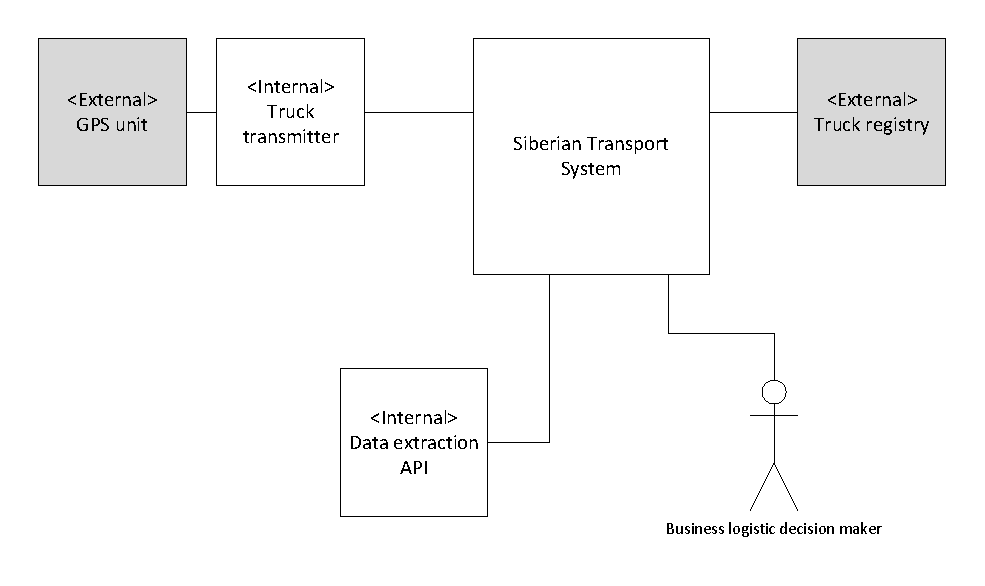
\includegraphics[width=\textwidth]{figures/sts_formal_context_diagram}\\
\end{center}
  \mycaption{Context diagram with information of externat and internal parts }

\begin{itemize}
\item The truck transmitters consist of a GPS unit, that gathers the trucks coordinates, and a sender unit, which will send the coordinates to our servers through a mesh-network. The hardware is a commodity-bought external system, but the software on the sender unit is internal.
\item The truck register is a system in which the Siberian trucking company's trucks are registered.  All the trucks will already be registered in this system, so data is imported from here to STS.  In the scope of our project, the truck register is an external system.  The trucks register sends a message to STS whenever a truck is added to the fleet, removed from the fleet, or reaches one of STC's central depots.
\end{itemize}


\subsection{Interaction scenarios}
\label{sec:inter-scen}

\begin{center}
  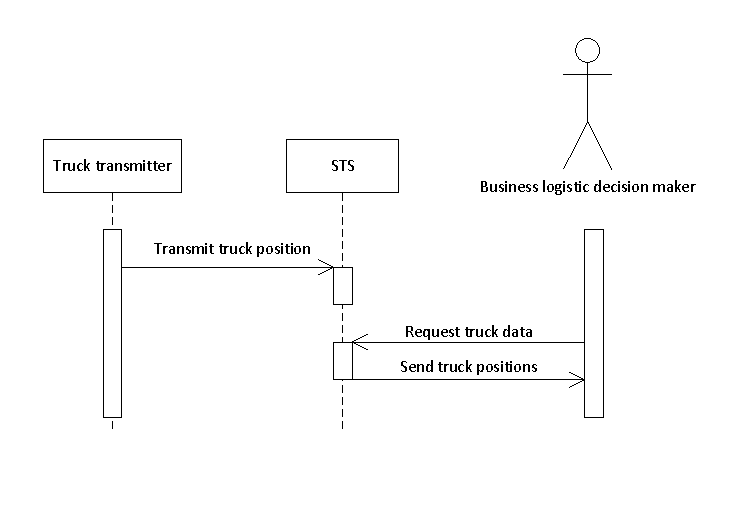
\includegraphics[width=\textwidth]{figures/interaction_scenario_1}\\
  \mycaption{Truck transmitters send positions to the server.  Later on, a user can make a query to see specific trucks or to see all trucks that fall behind schedule}
\end{center}



\section{Functional view}
\label{sec:functional-view}

\begin{center}
  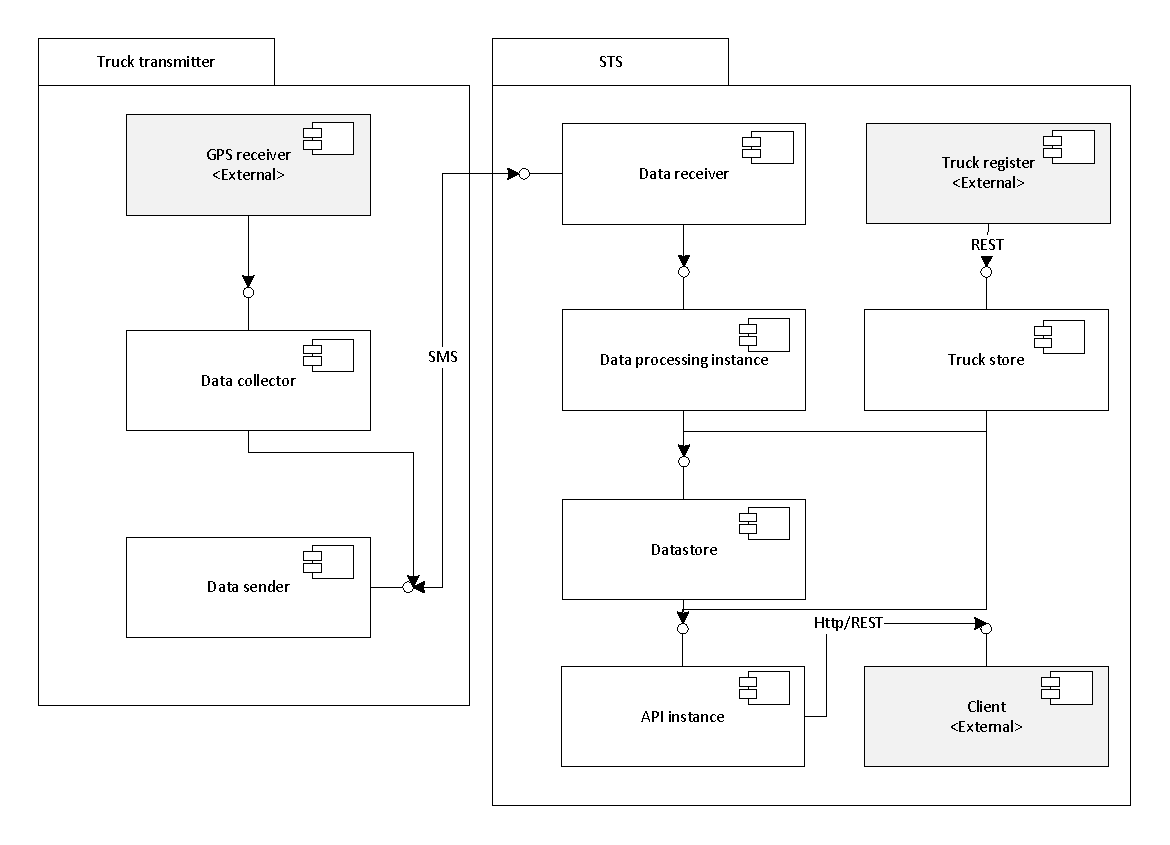
\includegraphics[width=\textwidth]{figures/functional_view}\\
  \mycaption{The figure shows the functional view for the truck transmitter and the Siberian Trucking System (STS) }
\end{center}


\instructions{
The functional view of the system defines the system’s architecturally
significant functional elements, the responsibilities of each, the
interfaces they offer and the dependencies between elements.

Place a functional model here (e.g. a UML component diagram) and
explain its content in the subsections below. A functional element is
a well-defined part of the runtime system that has particular
functional responsibilities and exposes interfaces that connect it to
other functional elements.


Focus on the important functional elements in your architecture. In
general you should not model the underlying infrastructure here unless
it performs a functionally significant purpose (for example a message
bus that links system elements and transforms data exchanged between
them).

If your architecture is functionally complex you may choose to model
it at a high level and then decompose some elements in further
sub-models (functional decomposition).

\begin{center}
  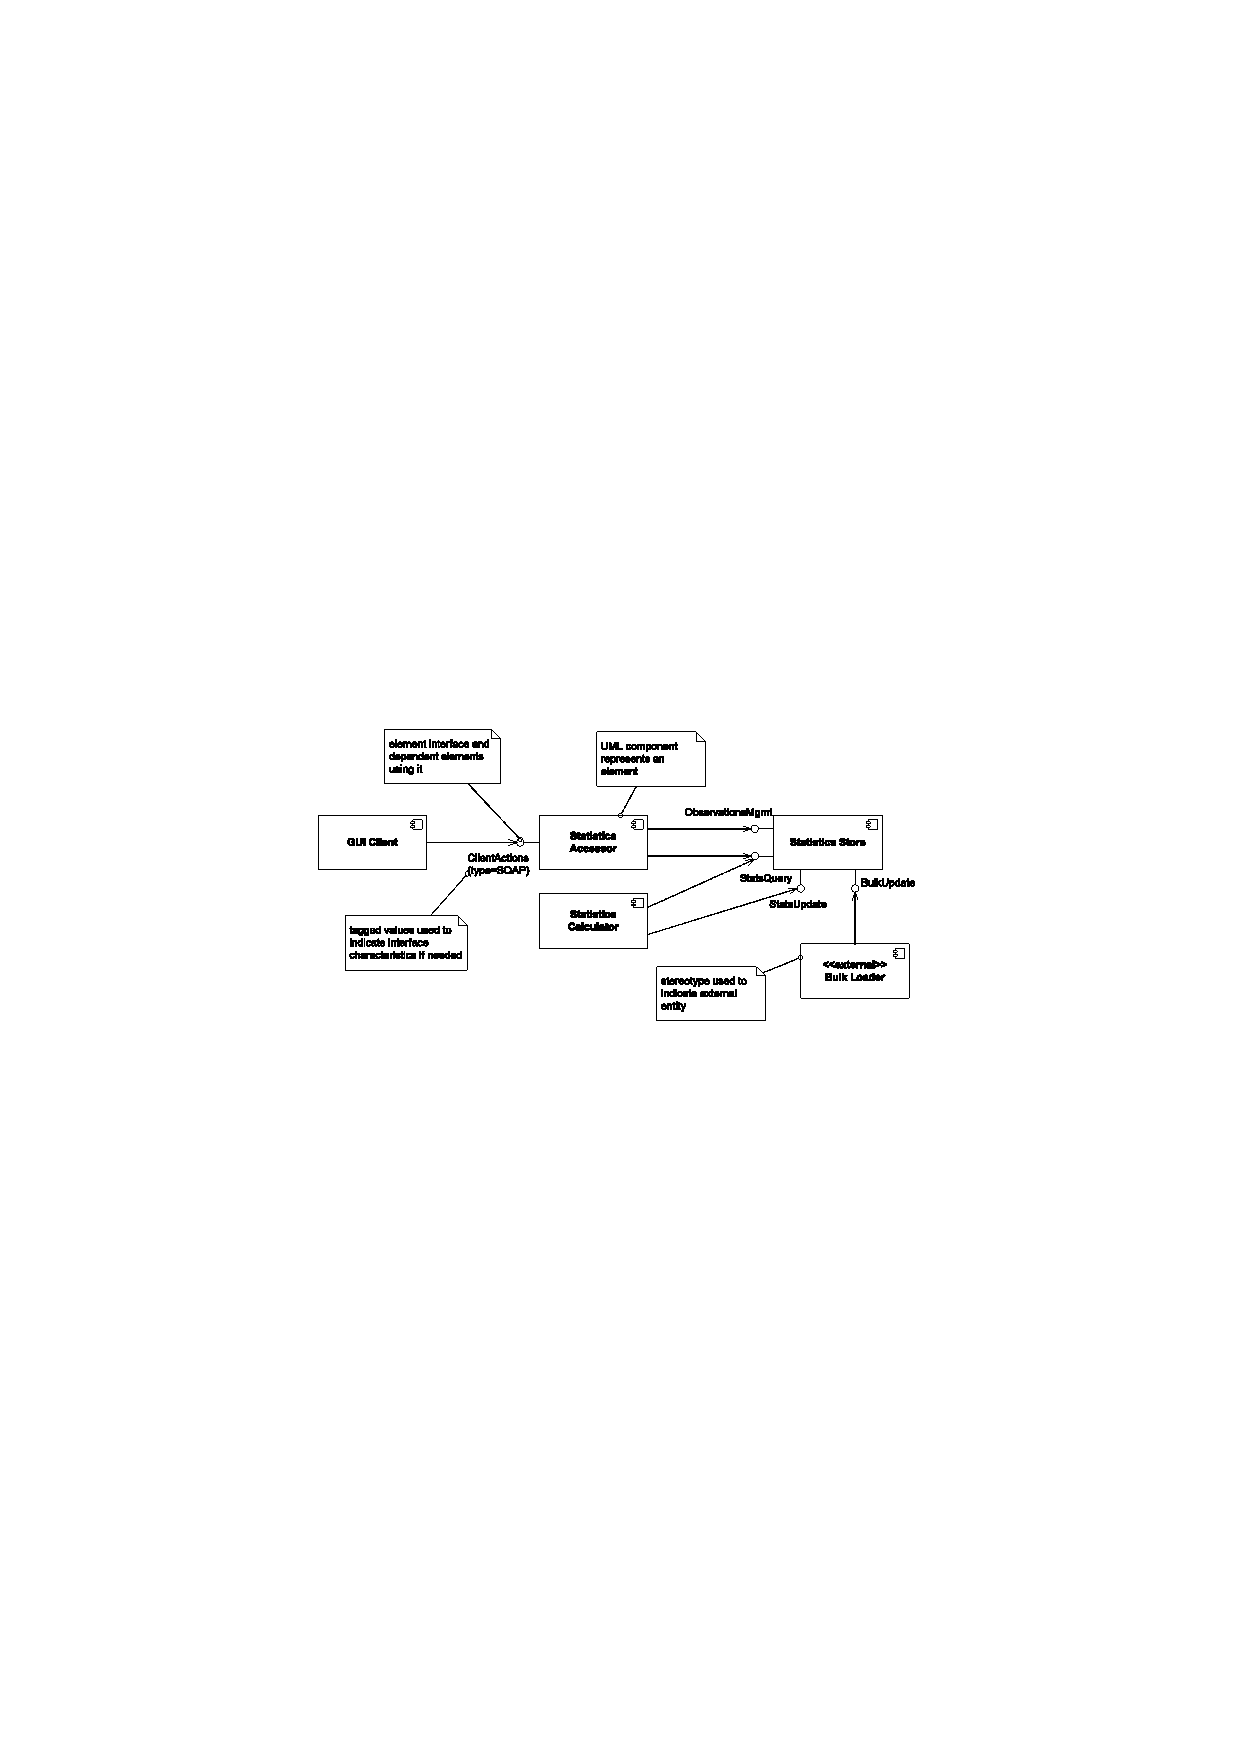
\includegraphics[width=\textwidth]{figures/functionalmodel}\\
  \mycaption{Functional model}
\end{center}

}

\subsection{Functional elements}
\label{sec:functional-elements}

\instructions{
Define the responsibilities and interfaces offered and/or required by
each functional element. Alternatively, if you are using a modelling
approach like UML you might choose to keep the main descriptions in
the UML model repository and summarise the information here,
referencing the model(s).

If you have used functional decomposition in the previous section, you
can structure this section to align with your functional hierarchy.

\begin{center}
  \begin{tabular}[h!]{| >{\columncolor{gray}}p{0.28\textwidth} | p{0.65\textwidth} |}
    \hline
    Element name & \\
    \hline
    Responsibilities & \\
    \hline
    Interfaces -- inbound & \\
    \hline
    Interfaces -- outbound & \\
   \hline
  \end{tabular}
\end{center}
}

\subsection{Functional scenarios}
\label{sec:functional-scenarios-1}

\instructions{
Use one or more interaction diagrams to explain how the functional
elements interact, via their interfaces, in order to meet some of the
key system functional scenarios.
}

\subsection{System-wide processing}
\label{sec:syst-wide-proc}

\instructions{
Define how any system-wide processing will be handled (for example, if
you have a message-oriented system, how will you deal with message
delivery errors across the system).
}

\section{Information view}
\label{cha:information-view}

\instructions{
The Information view of the system defines the structure of the
system’s stored and transient information (e.g. databases and message
schemas) and how related aspects such as information ownership, flow,
currency, latency and retention will be addressed.
}

\subsection{Data structure}
\label{sec:data-structure}

\instructions{
Define or reference any architecturally significant data structures
for stored and transient data, such as overview data models or message
schemas.

At this level you should keep the number of entities small – no more
than 20 or so if possible. It is not necessary to be 100\% normalised
– for the sake of clarity it is acceptable to have some many-to-many
relationships for example. Don’t try and illustrate every entity and
relationship here or your readers will get lost in the detail.

It may also be useful to logically group entities together that are
semantically related in some way – for example, all data related to
customer name and address. This may help your readers to understand
the data items and the relationships between them.

Here is an example data structure model which uses classic ERD
notation. You can also use class diagrams here although that may be
too granular a level of detail for an AD. An alternative, should you
wish to use UML, is to illustrate the information structure at the
package, rather than the class, level.

\begin{center}
  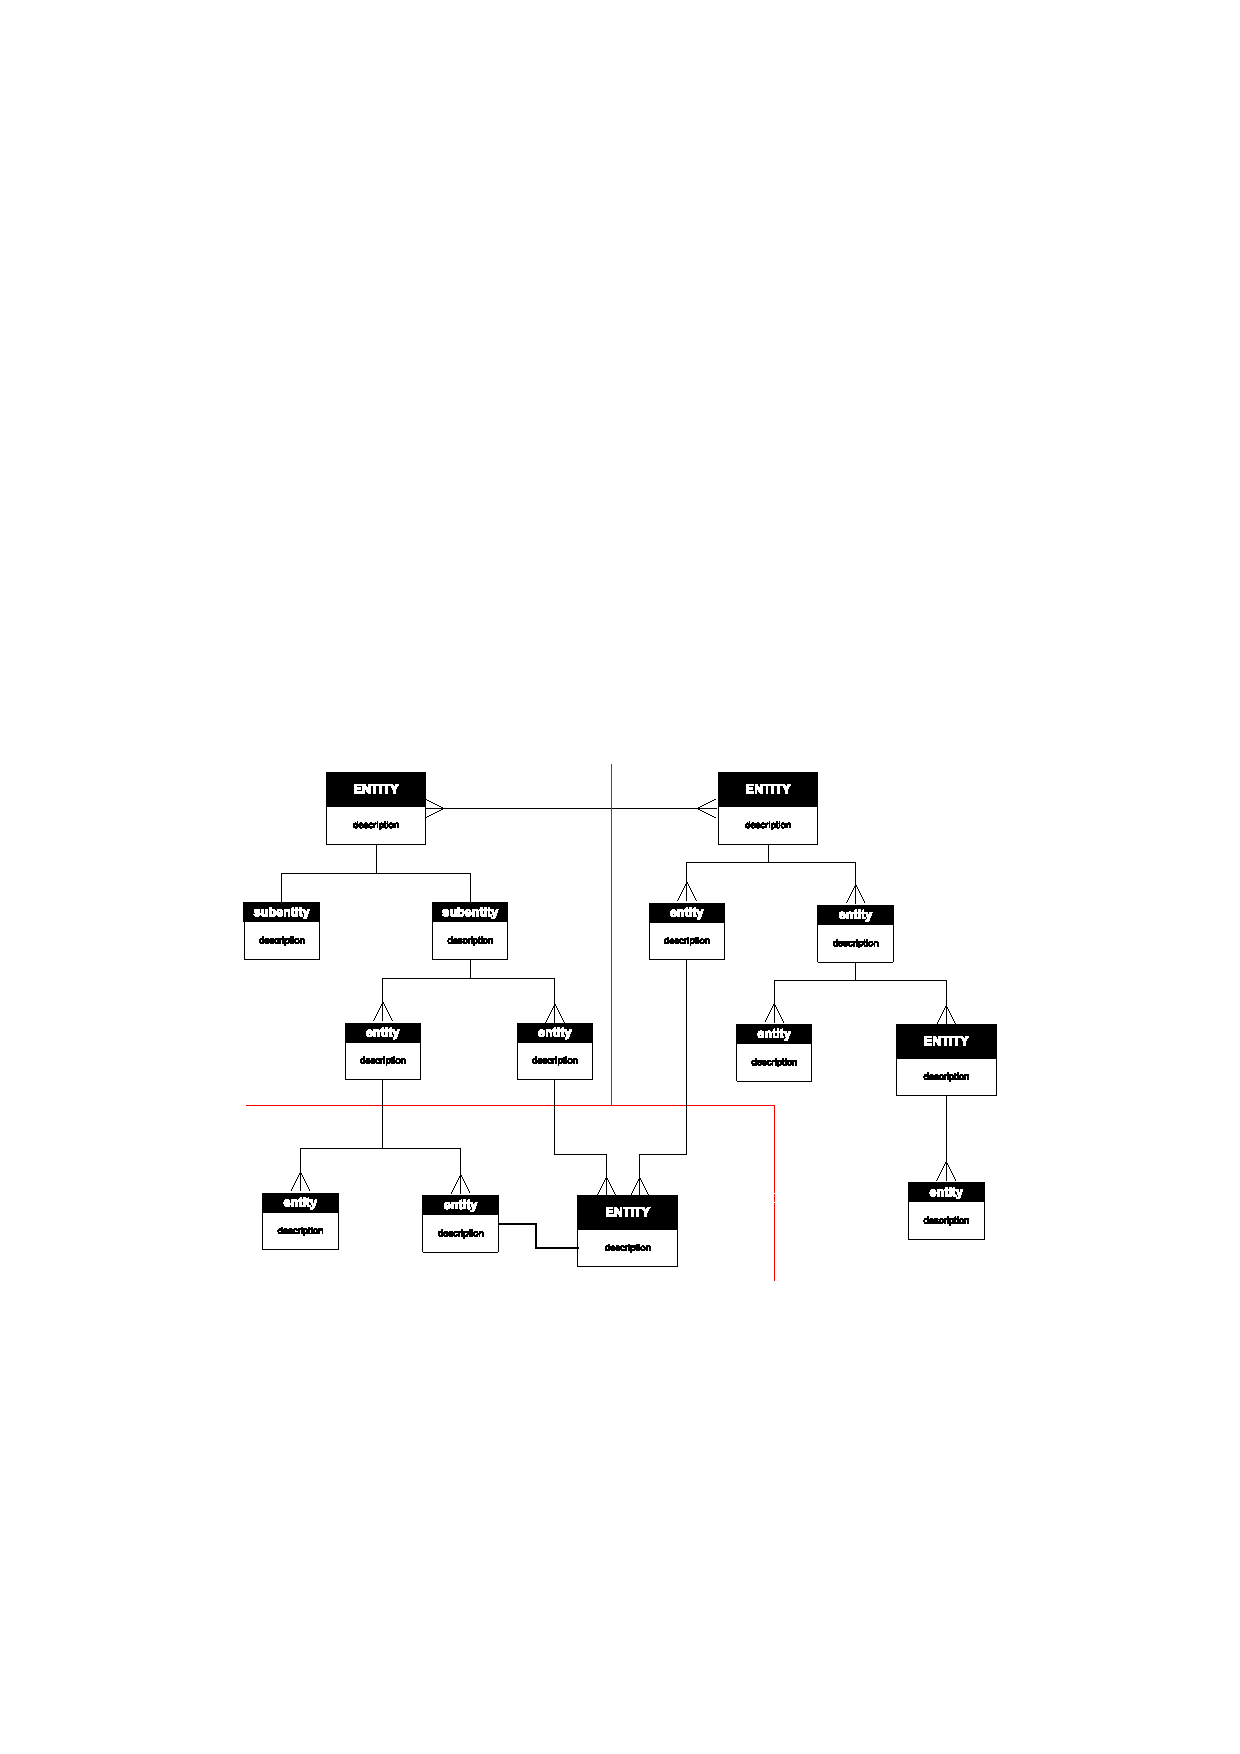
\includegraphics[width=\textwidth]{figures/systemdatastructure}\\
  \mycaption{System data structure}
\end{center}

}

\subsection{Data flow}
\label{sec:data-flow}

\instructions{
If it is not clear from the functional view’s interaction diagrams,
define how data flows through the system from one component to another
and to external components.

As with the data structure diagram, keep this simple and focus on no
more than about 10-15 key functional elements. Don’t try and
illustrate every data flow here or your readers will get lost in the
detail.

An example is shown below using a data flow diagram.

\begin{center}
  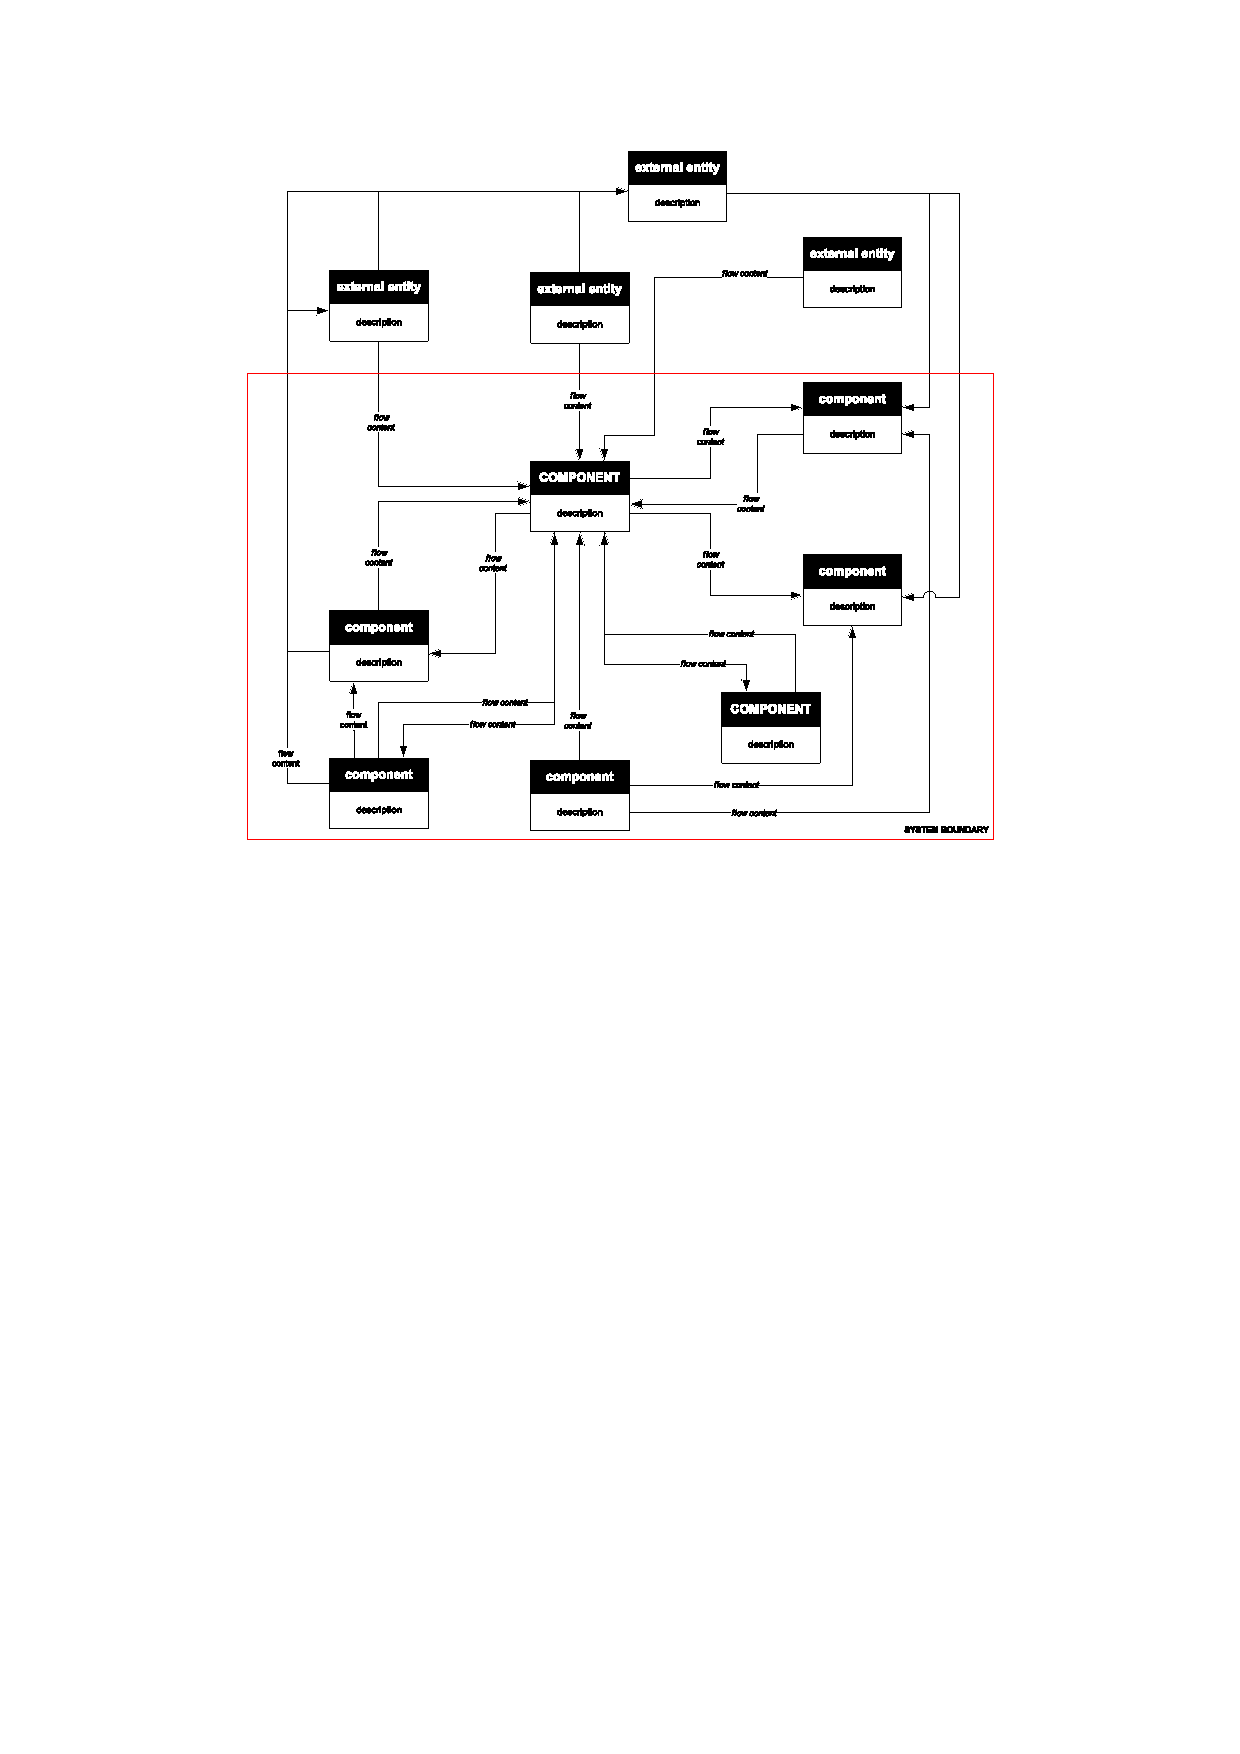
\includegraphics[width=\textwidth]{figures/systemdataflow}\\
  \mycaption{System data flow}
\end{center}
}

\subsection{Data ownership}
\label{sec:data-ownership}

\instructions{
If data is owned by more than one entity or part of the system, define
who owns which pieces of the data and explain how any resulting
problems will be handled.

In the example below, it can be seen that there are issues with entity
4 which can be updated by System D which is not the owner. The AD
should explain how this inconsistency will be managed.

\begin{center}
  \begin{tabular}[h!]{| p{0.1\textwidth} | p{0.15\textwidth} | p{0.15\textwidth} | p{0.15\textwidth} | p{0.15\textwidth} |}
    \hline
    \rowcolor{gray}
    Entity & System A & System B & System C & System D \\
    \hline
    \hline
    entity 1 & MASTER & r/o copy & reader  & reader \\
   \hline
    entity 2 &reader & MASTER & none & reader\\
   \hline
    entity 3 &none & reader & MASTER & reader \\
   \hline
    entity 4 &MASTER &none & none & reader, updater, deleter\\
   \hline
 \end{tabular}
\end{center}

}

\subsection{Information lifecycles}
\label{sec:inform-lifecycl}

\instructions{
If key entities have complicated lifecycles then model the way that
their state changes over time.

Focus on a few key entities whose transitions help to illuminate key
features of the architecture, rather than just
created / updated / updated / updated / destroyed.

There are two common techniques for modelling information lifecycles,
entity life histories and state transition diagrams. Both are useful;
choose one style and stick to it throughout the AD.

\begin{center}
  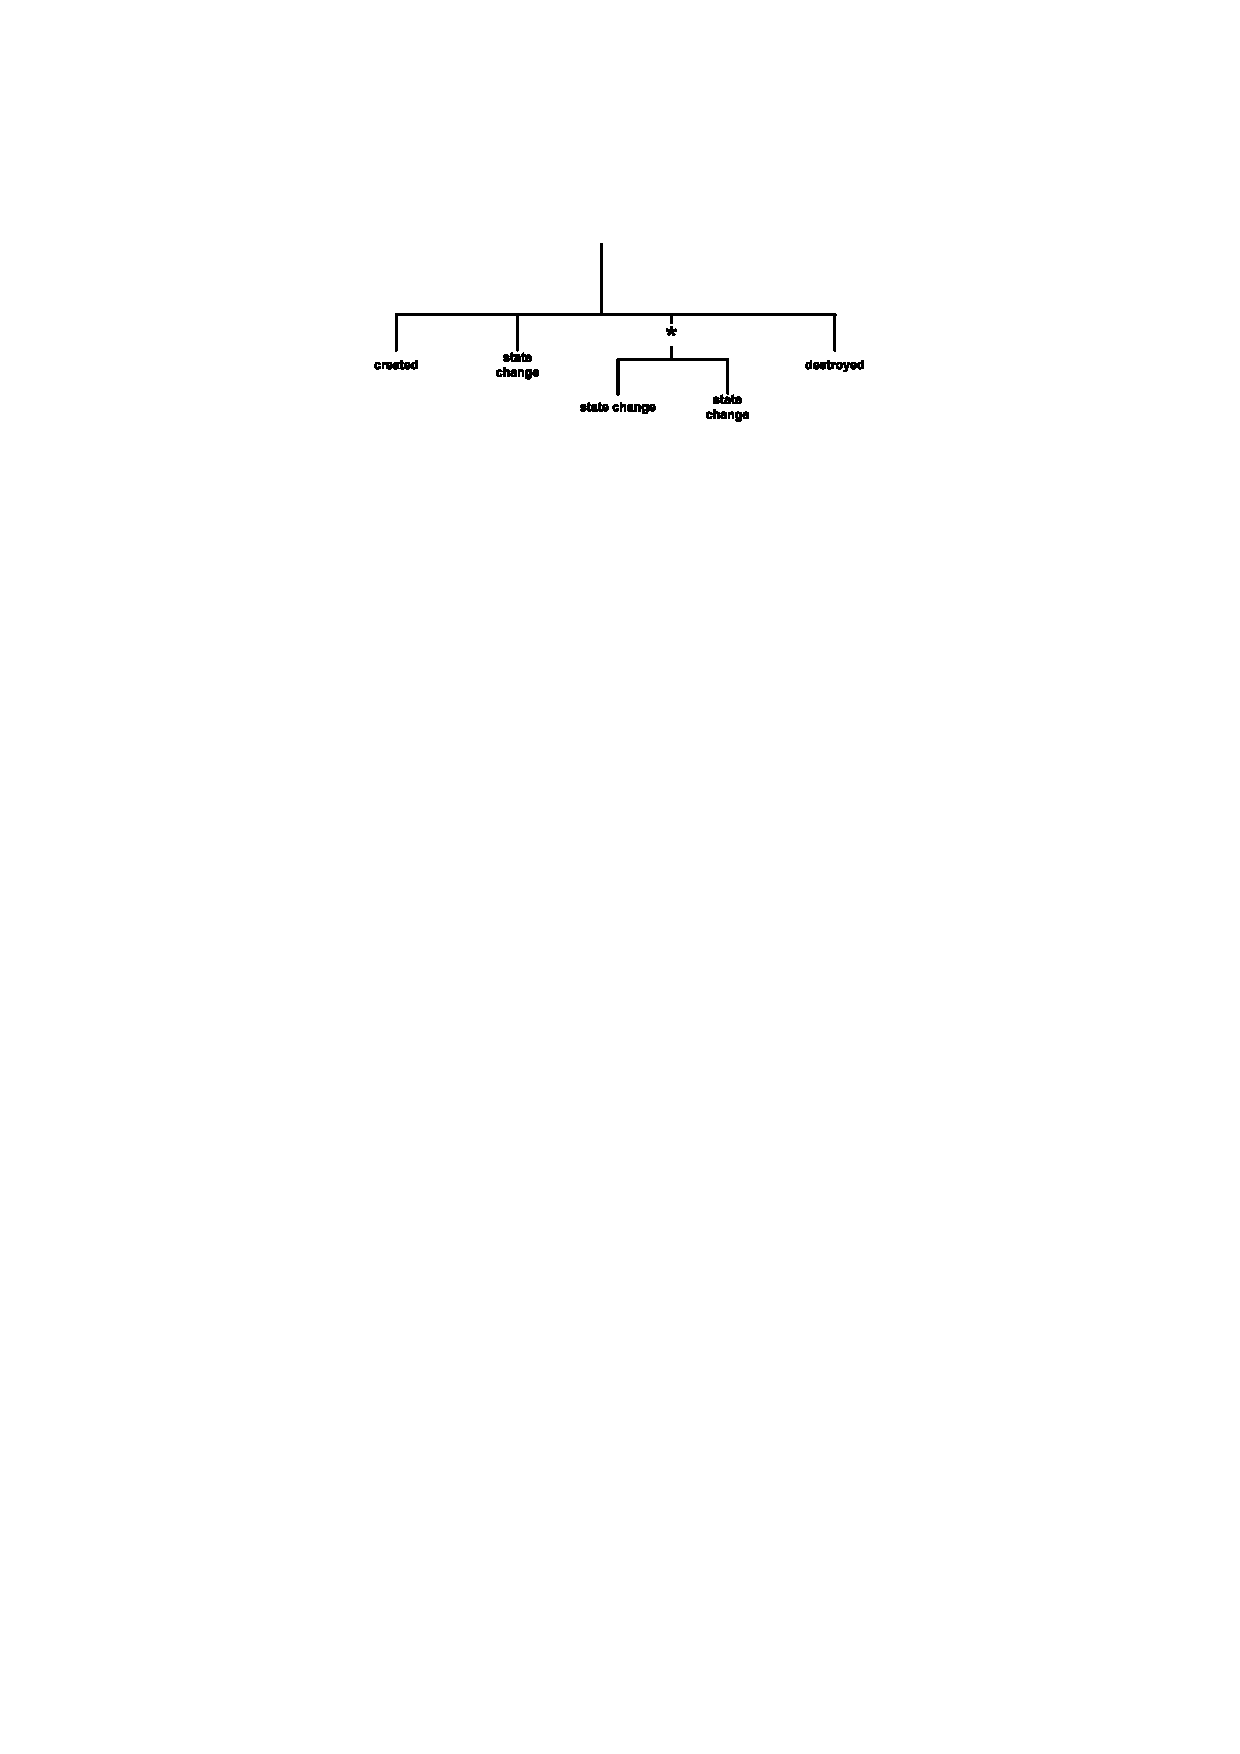
\includegraphics[width=0.7\textwidth]{figures/entitylifehistory}\\
  \mycaption{Entity life history}
\end{center}

\begin{center}
  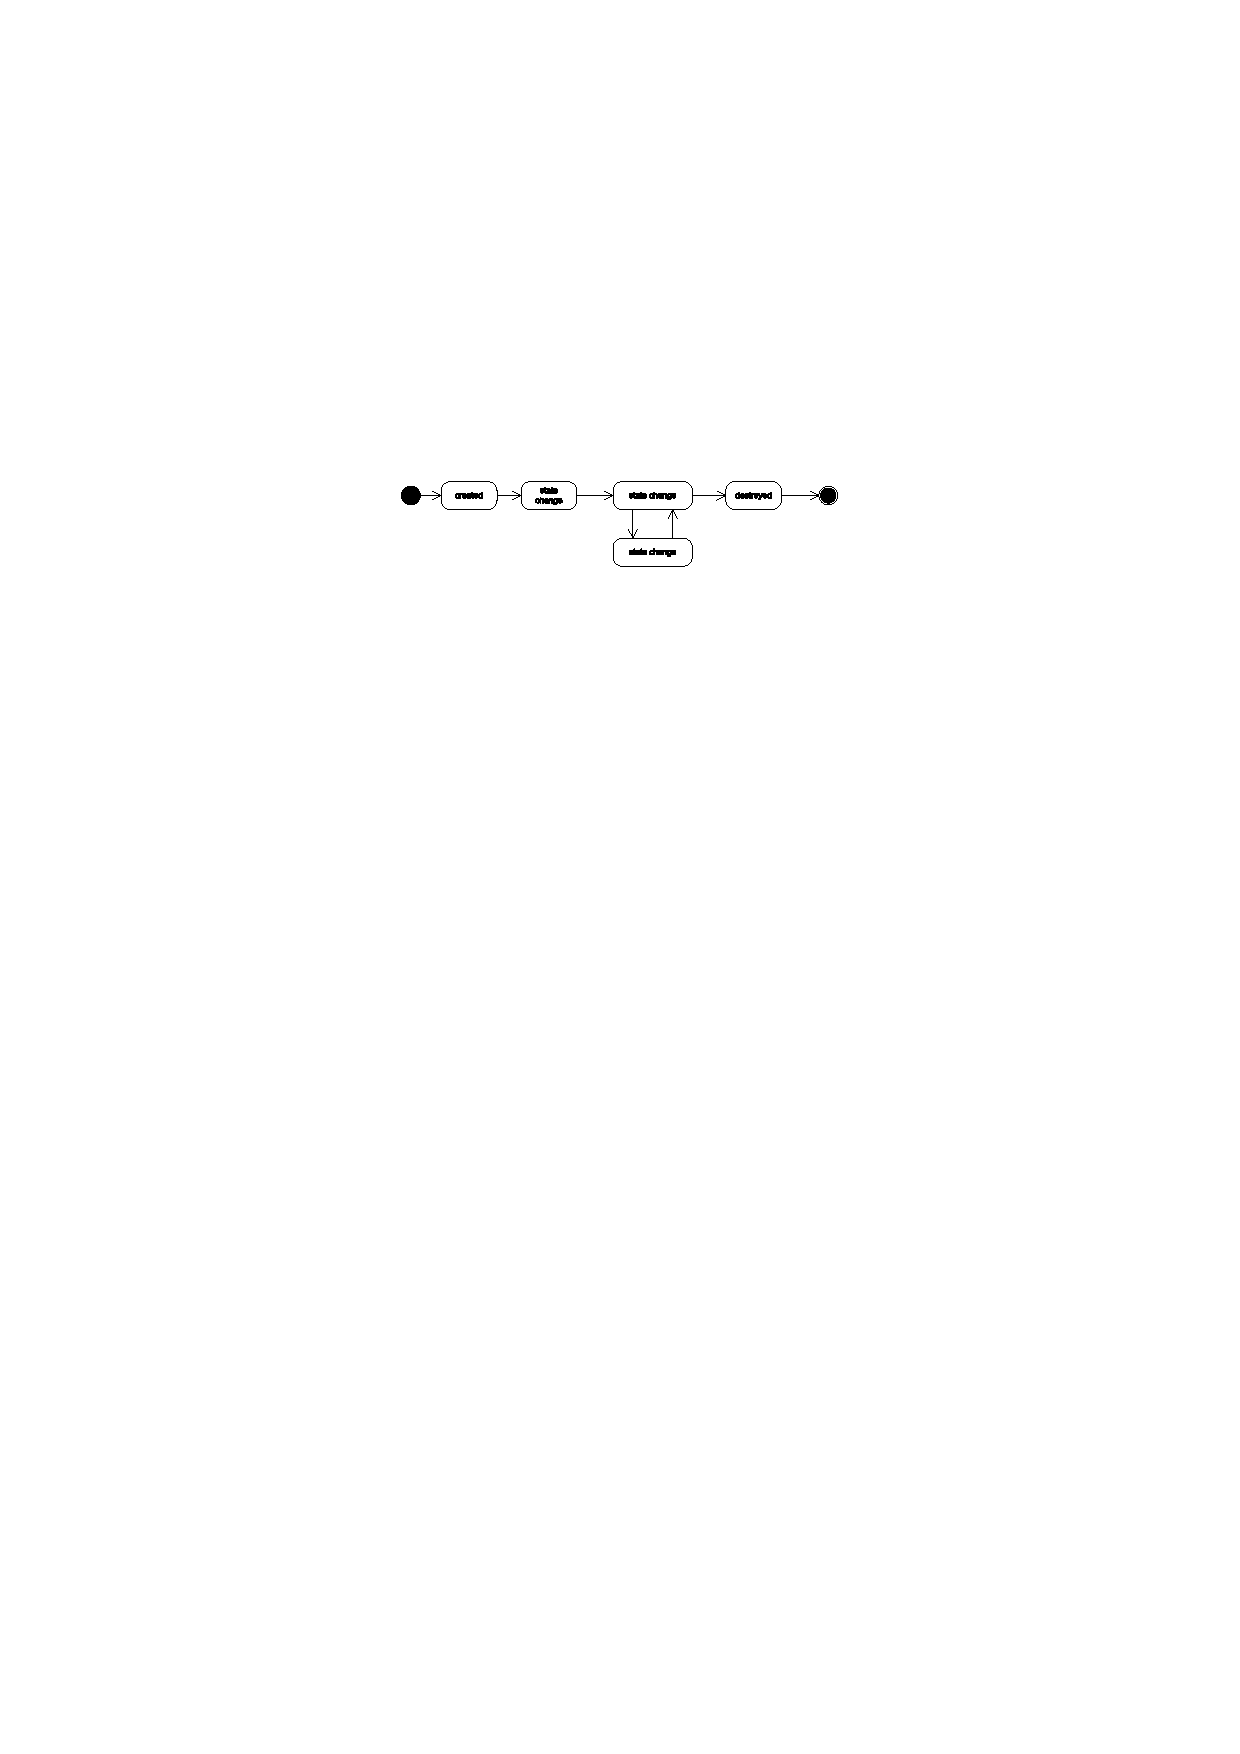
\includegraphics[width=0.7\textwidth]{figures/statetransition}\\
  \mycaption{State transition}
\end{center}

}

\subsection{Timeliness and latency}
\label{sec:timeliness-latency}

\instructions{
If information needs to be copied around the system or is updated
regularly, explain how timeliness and latency requirements will be
addressed.
}

\subsection{Archive and retention}
\label{sec:archive-retention}

\instructions{
Explain how will archive and retention requirements will be met by the
system.
}

\section{Concurrency view}
\label{sec:concurrency-view}

\instructions{
The Concurrency view of the system defines the set of runtime system
elements (such as operating system processes) into which the system’s
functional elements are packaged.

If the concurrency structure is complicated or it isn’t obvious from
the information in the other views, define how functional elements
will be packaged into processes and threads and explain how they
interact safely and reliably using suitable inter-process
communication mechanisms. This can be achieved via a UML model (using
stereotypes), by using a special purpose concurrency modelling
language, or by creating an informal notation for the situation at
hand.
}

\subsection{Concurrency model}
\label{sec:concurrency-model}

\instructions{
Model the processes, process groups and threads, and the interprocess
communication channels between them.

You may also choose to model the mechanisms used to protect the
integrity of data and other resources shared between concurrent
execution units, such as mutexes or semaphores.

You can use a UML component model to represent the information
graphically, stereotyping the components appropriately.

\begin{center}
  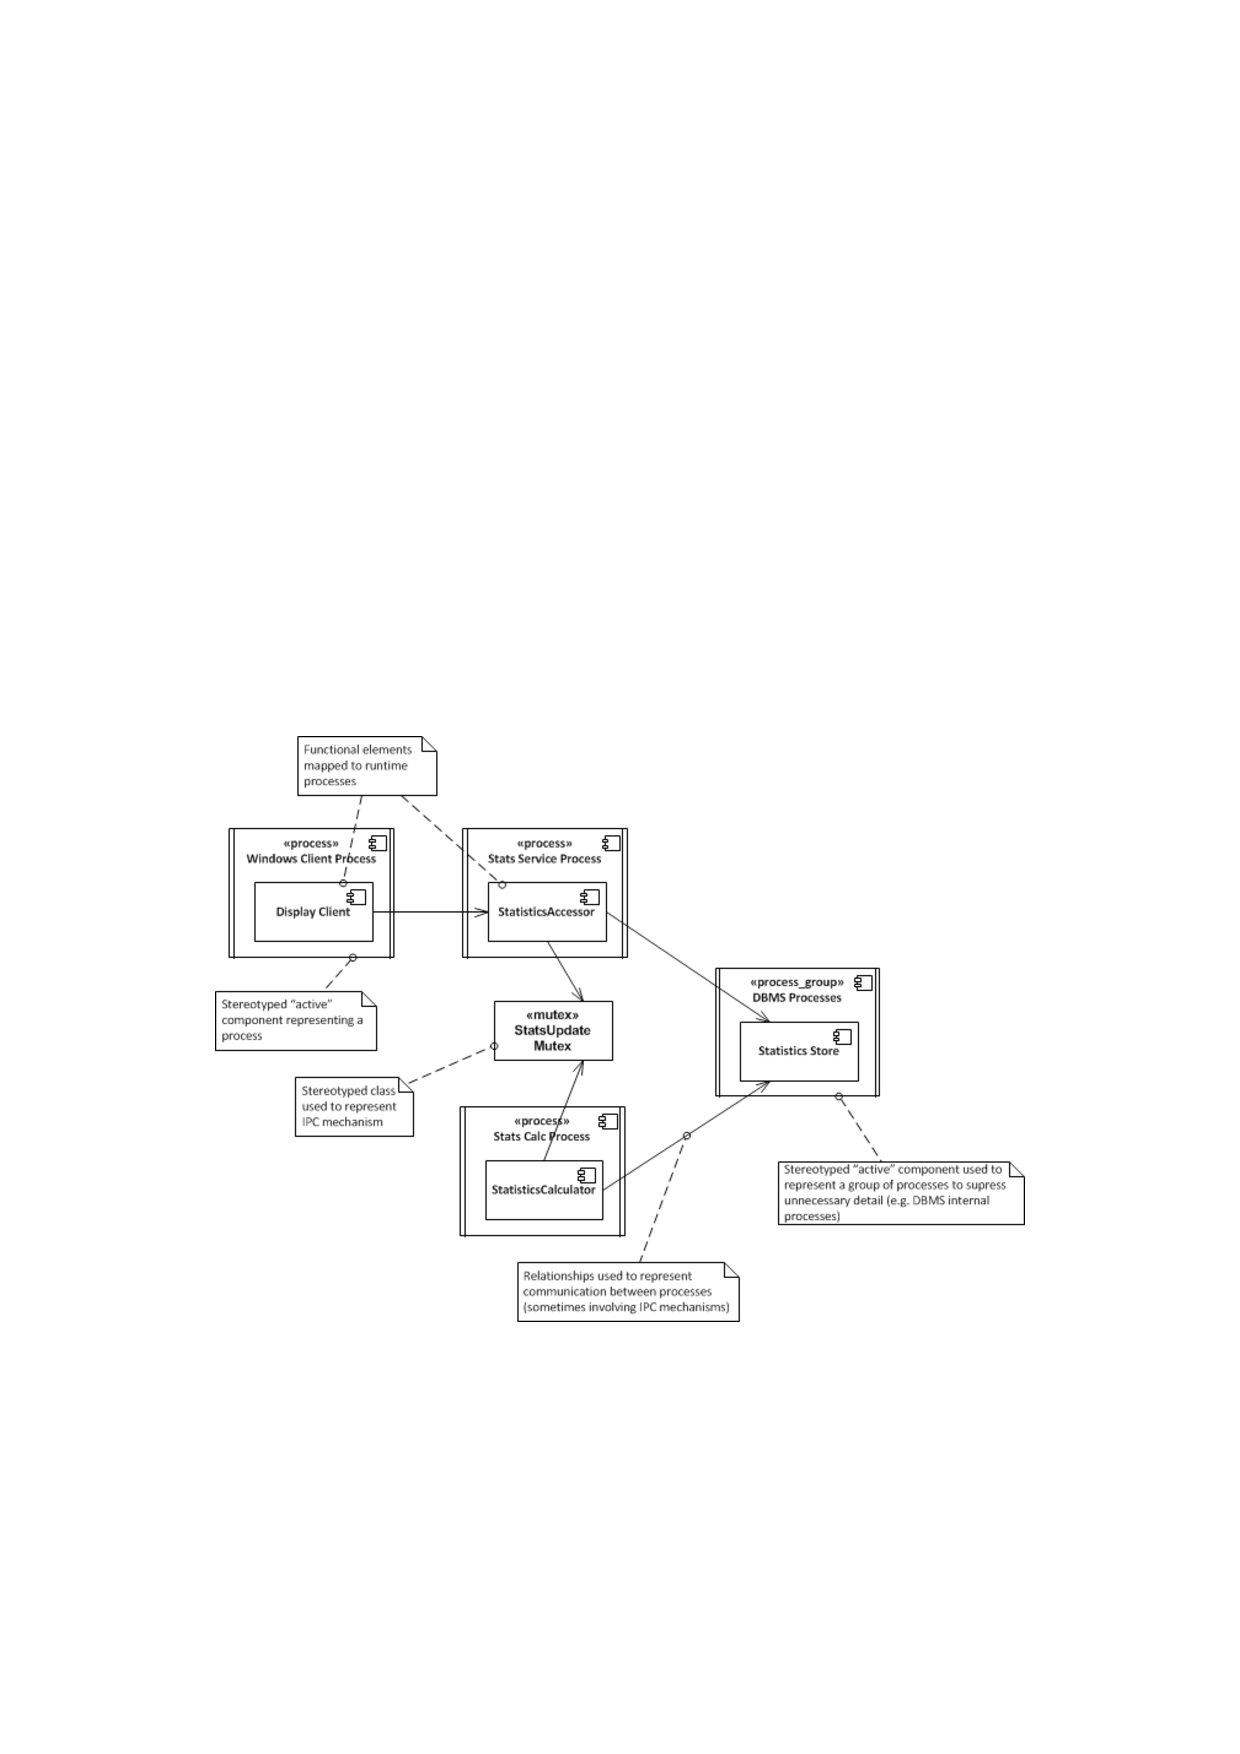
\includegraphics[width=\textwidth]{figures/concurrencymodel}\\
  \mycaption{Concurrency model}
\end{center}

}

\subsection{State model}
\label{sec:state-model}

\instructions{
Model the states that the systems runtime elements can be in, the
transitions between those states and the events which drive those
transitions.

A state is an identified, named stable condition which occurs during
the system’s runtime. An event is something that happens which causes
an element to undergo a transition from one state to another. Actions
may also be associated with transitions, so that while the element
changes state, the action is performed.

Focus on a few key elements whose states and transitions help to illuminate
key features of the architecture.

\begin{center}
  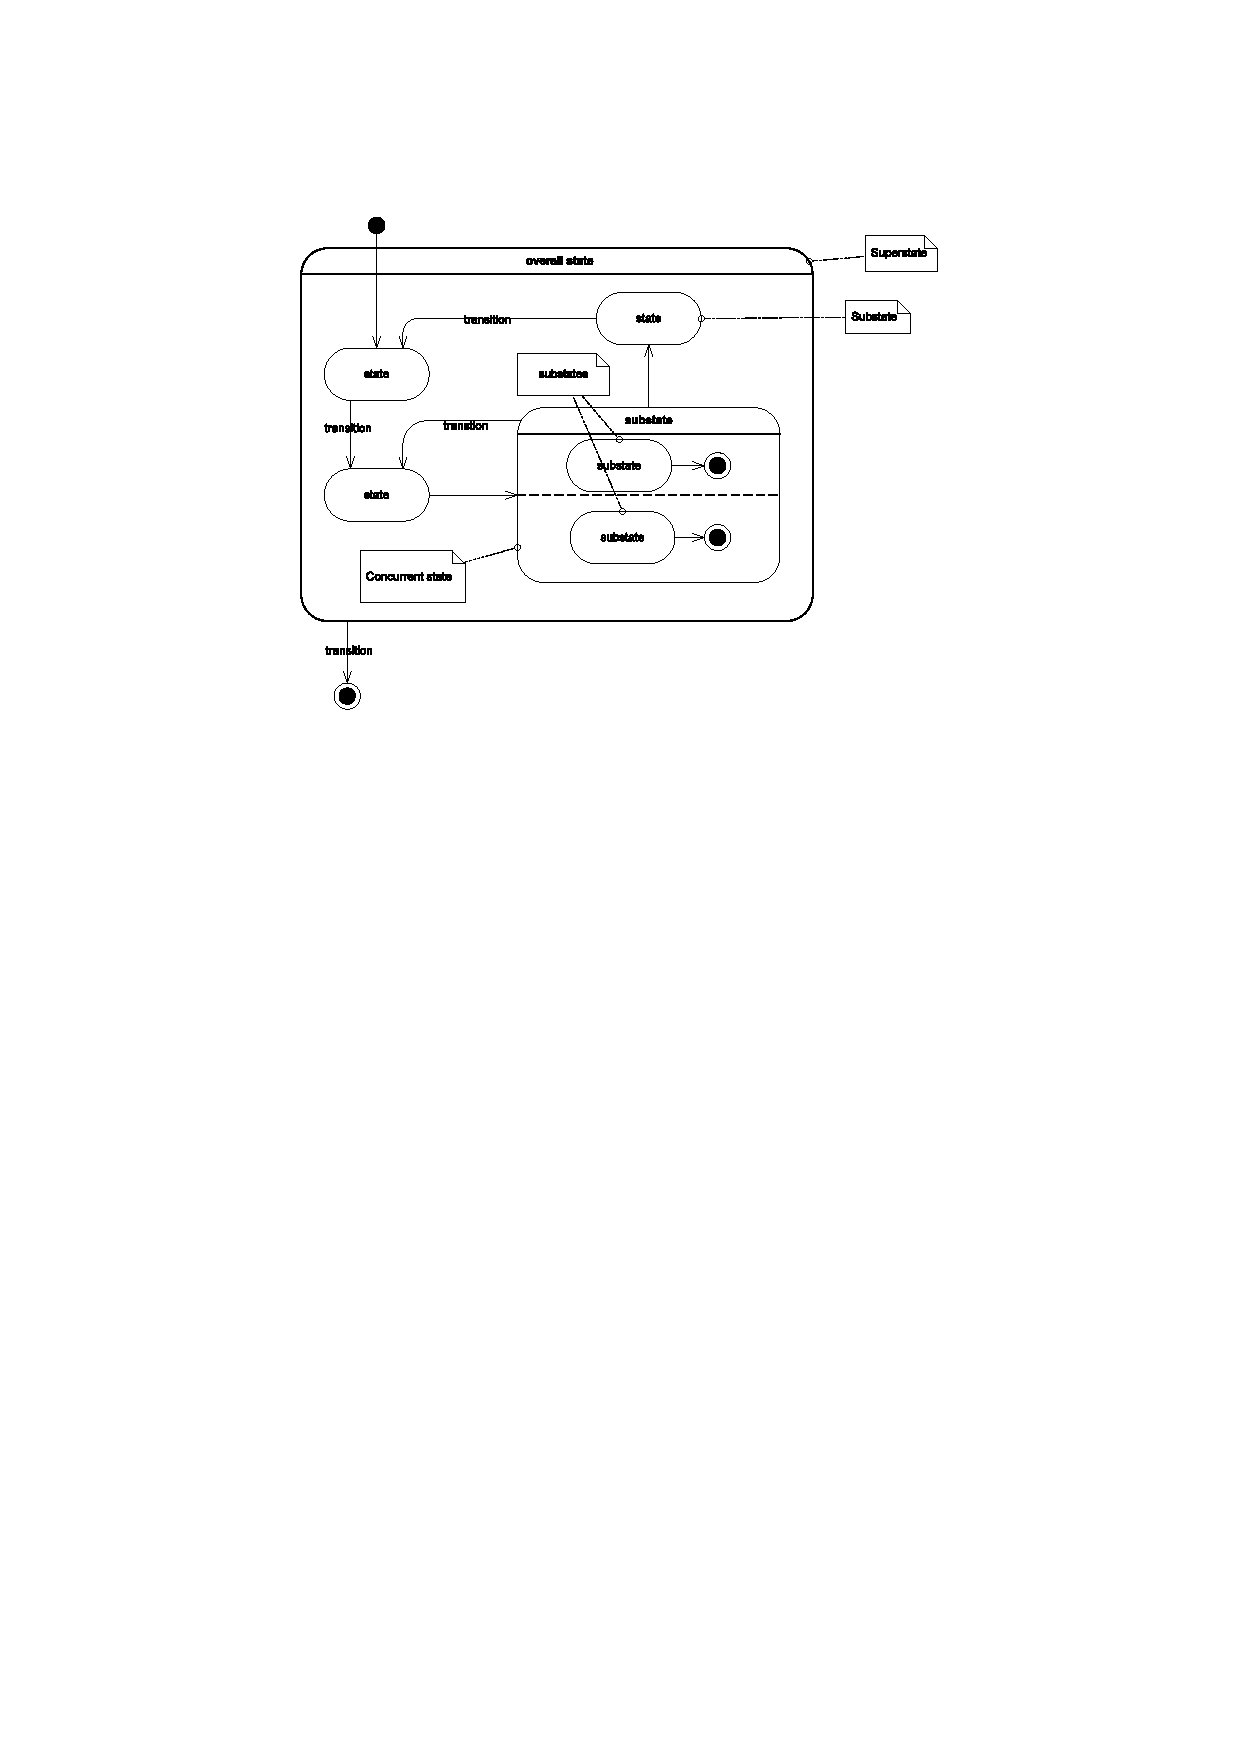
\includegraphics[width=0.8\textwidth]{figures/statemodel}\\
  \mycaption{State model}
\end{center}

}

\section{Deployment view}
\label{sec:deployment-view}

\instructions{
The Deployment view of the system defines the important
characteristics of the system’s operational deployment
environment. This view includes the details of the processing nodes
that the system requires for its installation (i.e. its runtime
platform), the software dependencies on each node (such as required
libraries) and details of the underlying network that the system will
require.
}

\subsection{Runtime platform model}
\label{sec:runt-platf-model}

\instructions{
Show the system’s runtime platform (defining nodes, links and the
mapping of functional elements or processes to nodes).

You can use a UML deployment diagram here, or a simpler
boxes-and-lines diagram.

\begin{center}
  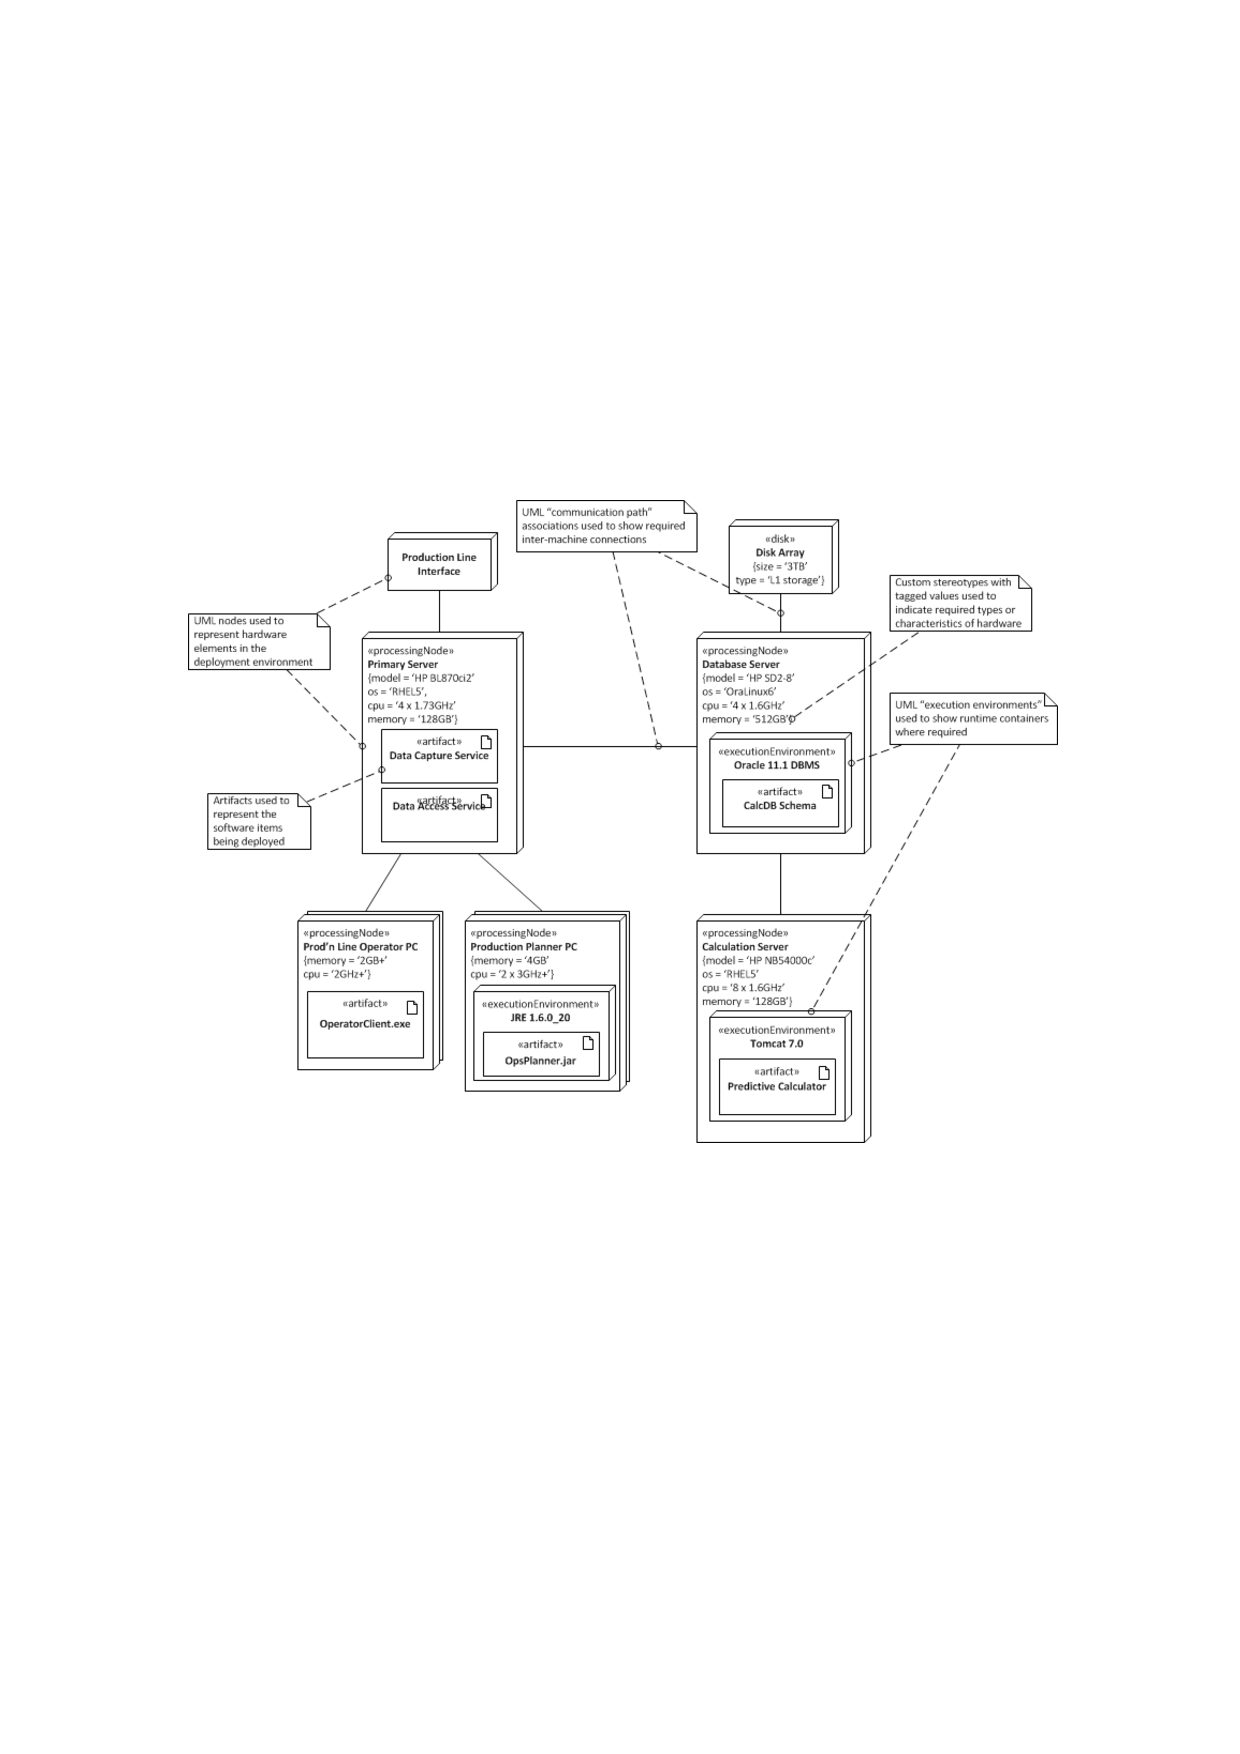
\includegraphics[width=\textwidth]{figures/deploymentmodel}\\
  \mycaption{Deployment model}
\end{center}

}

\instructions{
It is often useful to explicitly map the functional elements onto the
nodes that they will be running on, particularly if the deployment
model is complex or the mappings aren’t obvious.

\begin{center}
  \begin{tabular}[h!]{| p{0.4\textwidth} | p{0.5\textwidth} |}
    \hline
    \rowcolor{gray}
    Functional element & Deployment node(s) \\
    \hline
    \hline
    & \\
    \hline
    & \\
    \hline
  \end{tabular}
\end{center}

}

\subsection{Software dependencies}
\label{sec:softw-depend}

\instructions{
Define the software that will be required on the various types of node
in the runtime platform model, in order to support the system (such as
operating system , system software or library requirements). Where
versions are known you should state these.

Clearly state any known version dependencies (eg component A requires
at least version X of component B).

This can usually be presented in tabular form.
}

\subsection{Network model}
\label{sec:network-model}

\instructions{
If network requirements are complex, include a network model that
illustrates the nodes, links and network hardware that the system
requires, making quality of service requirements clear.
}

\section{Development view}
\label{sec:development-view}

\instructions{
The Development view of the system defines any constraints on the
software development process that are required by the
architecture. This includes the system’s module organisation, common
processing that all modules must implement, any required
standardisation of design, coding and testing and the organisation of
the system’s codeline.

Much of the information in this view is normally presented at a
summary level, with more detail being available in other developer
focused documents such as a development standards document. However
you may still need to record some architecturally significant
decisions at this stage, for example around choice of libraries or
frameworks, or approach and tools for software deployment or
configuration management.
}

\subsection{Module structure}
\label{sec:module-structure}

\instructions{
Use a model that defines the code modules that will be created and the
dependencies between them. A UML package diagram is often an effective
way to achieve this.

\begin{center}
  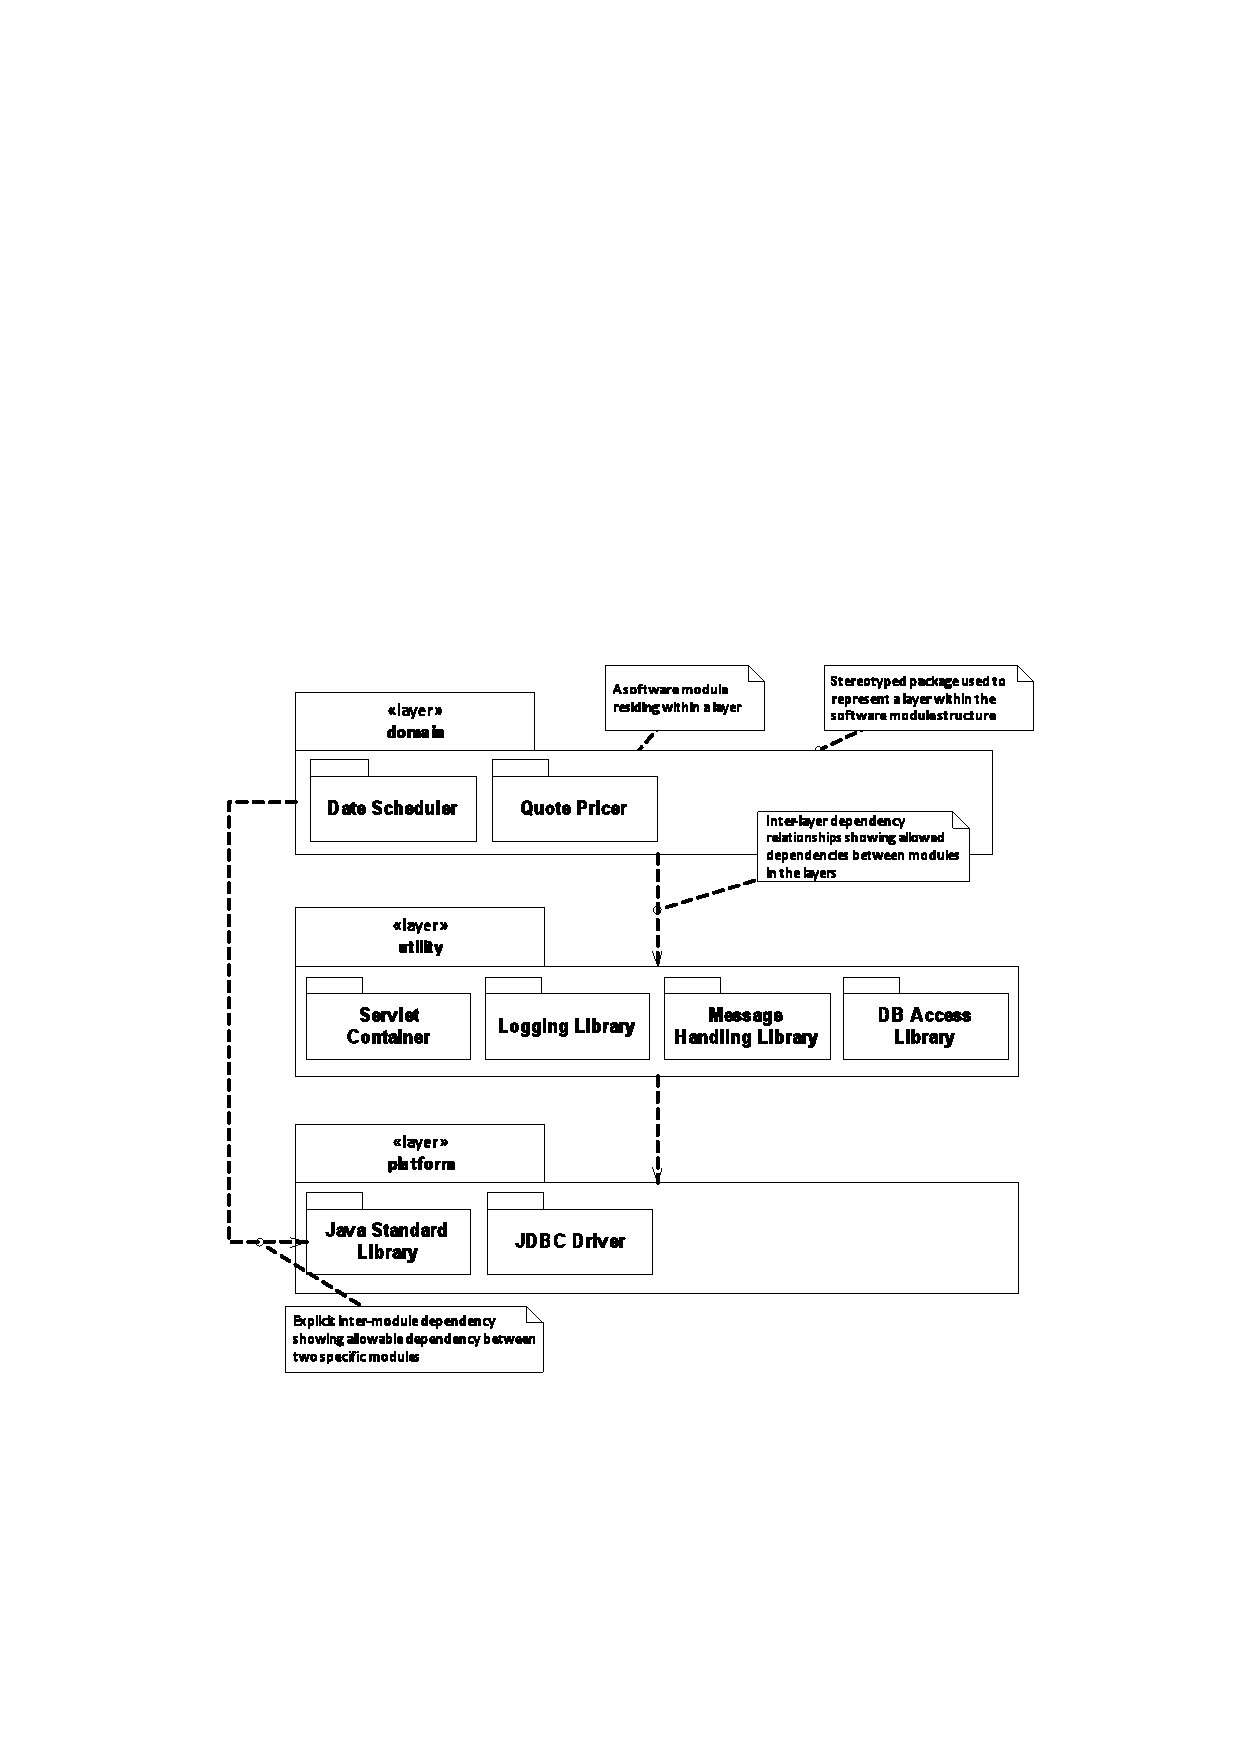
\includegraphics[width=0.9\textwidth]{figures/modulestructurediagram}\\
  \mycaption{Module structure diagram}
\end{center}

}

\subsection{Common design}
\label{sec:common-design}

\instructions{
Define the common design (such as logging, security, tracing and so
on) that must be performed in a standard way across the system and how
it should be performed (e.g. via a design pattern or reference to a
code library or sample).
}

\subsection{Standards for design, code, and test}
\label{sec:stand-design-code}

\instructions{
Define any standards that must be followed for design, code and unit
testing, probably by reference to an external document.
}

\subsection{Codeline organization}
\label{sec:codel-organ}

\instructions{
Define the codeline structure (i.e. how the source code will be held
as a directory hierarchy and how it will be built into deliverable
software). Define the directory hierarchy, build tools and delivery
tools (such as testing or continual integration tools) that will be
used to deliver the software for testing and production.
}

\section{Operational view}
\label{sec:operational-view}

\instructions{
The Operational view defines how the system will be installed into its
production environment, how data and users will be migrated to it and
how it will be configured, managed, monitored, controlled and
supported once this is achieved. The aim of the information in this
view is to show how the operational environment is to be created and
maintained, rather than to define detailed instructions or procedures.
}
\subsection{Installation and migration}
\label{sec:inst-migr}

\instructions{
Define the high-level steps required to install the system and any
specific or unusual requirements for it.

If parallel running of old and new systems is required, explain how
this will be done without disrupting existing systems, and the
transition states required.
}

\subsection{Operational configuration management}
\label{sec:oper-conf-manag}

\instructions{
Define the main groups of operational configuration items and common
sets of values for them (e.g. batch and overnight sets) and explain
how these groups will be managed in the production environment.
}

\subsection{System administration}
\label{sec:syst-admin}

\instructions{
Explain the requirements the system places on the systems
administrators (in both routine and exceptional situations) and the
facilities that the system will provide or rely on in the operational
environment.
}

\subsection{Provision of support}
\label{sec:provision-support}

\instructions{
Define the groups involved in providing support for the system and the
roles and responsibilities of each (including escalation procedures if
relevant).
}

\chapter{System qualities}
\label{cha:system-qualities}
\thispagestyle{fancy}

\instructions{
This section explains how the architecture presented
  meets its each of its required system quality properties.

While much of this information will be intrinsic to the views
documented in the previous chapter, it is often useful to bring out
some of it separately. In particular, if a quality property such as
security or performance depends on features documented in several
different views, then you should explain this here. For example,
scalability may depend on optimisations in the data model (documented
in the Information View) along with load balancing components
(documented in the Deployment View).
}

\section{Performance and scalability}
\label{sec:perf-scal}

\instructions{
For each of the main performance and scalability requirements, explain
how the system will meet the requirement. Refer to practical testing
and performance modelling work that has been performed as part of
applying this perspective.

\begin{center}
  \begin{tabular}[h!]{| p{0.4\textwidth} | p{0.5\textwidth} |}
    \hline
    \rowcolor{gray}
    Requirement & How met \\
    \hline
    \hline
    1. average user response time should be XX under load YY & refer
    to performance modelling spreadsheet\\

    \hline
 \end{tabular}
\end{center}

}

\section{Security}
\label{sec:security}

\instructions{
For each of the main, security requirements, explain how the system
will meet the requirement. Define (or reference) the threat model,
security policy and security design that have been used as part of
applying this perspective.

\begin{center}
  \begin{tabular}[h!]{| p{0.4\textwidth} | p{0.5\textwidth} |}
    \hline
    \rowcolor{gray}
    Requirement & How met \\
    \hline
    \hline
    1. all users must be authenticated before being allowed to access
    the system & access to all screens is via standard login screen
    with passwords synchronised overnight to central LDAP service\\

    \hline
 \end{tabular}
\end{center}

}


\section{Availability and resilience}
\label{sec:avail-resil}

\instructions{
Explain the A\&R requirements.

Define the availability schedule(s) for the system.

Explain how the system will meet the requirements, referring to
practical testing, modelling and design work that has been performed
as part of applying this perspective.

\begin{center}
  \begin{tabular}[h!]{| p{0.4\textwidth} | p{0.5\textwidth} |}
    \hline
    \rowcolor{gray}
    Requirement & How met \\
    \hline
    \hline
    1. There should be no single point of failure & all deployment
    nodes are clustered or load-balanced; where nodes are clustered,
    component failure is detected automatically and the passive node
    is brought up automatically\\

    \hline
 \end{tabular}
\end{center}

}


\section{Evolution}
\label{sec:evolution}

\instructions{
Explain the evolution requirements.

Define the evolutionary dimensions that are relevant to the system.

Explain  how the system will meet the requirements, taking into
account the likelihood of each type of evolution occurring (explaining
how the probabilities were arrived at) and referring to the design
work performed as part of applying his perspective.

\begin{center}
  \begin{tabular}[h!]{| p{0.4\textwidth} | p{0.5\textwidth} |}
    \hline
    \rowcolor{gray}
    Requirement & How met \\
    \hline
    \hline
    1. it must be possible to add extra input channels without having
    to redesign the core system & input channel components are loosely
    coupled to central processing modules via standardises abstract
    interfacey\\

    \hline
 \end{tabular}
\end{center}
}

\section{Other qualities}
\label{sec:other-qualities}

\subsection{Accessibility}
\label{sec:accessibility}

\instructions{
Explain how the system meets any accessibility requirements (if any).
}

\subsection{Internationalisation}
\label{sec:internationalisation}

\instructions{
Explain how the system meets any internationalisation (or
localisation) requirements (if any).
}

\subsection{Location}
\label{sec:location}

\instructions{
Explain how the system meets any requirements for the geographical
location(s) it is to be installed in (if any).
}

\subsection{Regulation}
\label{sec:regulation}

\instructions{
Explain how the system meets any regulatory requirements (if any).
}

\subsection{Usability}
\label{sec:usability}

\instructions{
Explain how the system meets any usability requirements (if any).
}

\appendix

\chapter{Architecture backlog}
\label{cha:architecture-backlog}
\thispagestyle{fancy}

\instructions{ Maintain a \emph{backlog} listing needs you have,
  issues and problems you have to solve, ideas for future design
  decisions etc. Note actions that you need to take and update the
  backlog as actions are completed:

\bigskip
Actions

\begin{itemize}
\item Decide on which Android version to target
\item ...
\end{itemize}

Done

\begin{itemize}
\item Create an architectural prototype using java.nio for increased
  scalability

\end{itemize}


}

\chapter{Architecture evaluation}
\label{cha:arch-eval}
\thispagestyle{fancy}

\instructions{
Describe the architectural evaluation that you performed, cf. Chapter
14 of~\citet{rozanski2011software} including what you learned about
your architecture design.
}

\chapter{Architecture skeleton}
\label{cha:arch-prot}
\thispagestyle{fancy}
\instructions{ 
Describe the architecture skeleton that you developed
  including how to download and run it.
}





% 
% Bibliography
% 
\bibliography{architectural_design}
\bibliographystyle{apalike}

\end{document}
